\documentclass[xcolor=svgnames,9pt,english,aspectratio=169,t]{beamer}
%\documentclass[xcolor=svgnames,9pt,english,handout,aspectratio=169,t]{beamer}
\newcommand{\handout}{0}

% =====================================================================
% POLI 450A (2026) --- shared TEMPLATE layer.
%
% Input from each lecture near the top of its file, BEFORE
% ../course_theme.tex (metropolis must be selected before the course
% palette overrides it):
%
%   \documentclass[xcolor=svgnames,9pt,english,aspectratio=169]{beamer}
%   \newcommand{\handout}{0}
%   % =====================================================================
% POLI 450A (2026) --- shared TEMPLATE layer.
%
% Input from each lecture near the top of its file, BEFORE
% ../course_theme.tex (metropolis must be selected before the course
% palette overrides it):
%
%   \documentclass[xcolor=svgnames,9pt,english,aspectratio=169]{beamer}
%   \newcommand{\handout}{0}
%   % =====================================================================
% POLI 450A (2026) --- shared TEMPLATE layer.
%
% Input from each lecture near the top of its file, BEFORE
% ../course_theme.tex (metropolis must be selected before the course
% palette overrides it):
%
%   \documentclass[xcolor=svgnames,9pt,english,aspectratio=169]{beamer}
%   \newcommand{\handout}{0}
%   \input{../course_preamble.tex}
%   \input{../course_theme.tex}
%   \graphicspath{{./}{./figs/}}
%   \title[Short title]{450A Political Methodology I}
%   \subtitle{Lecture N: ...}
%
% Modeled on the 2026 Northwestern workshop template
% (Teaching/PanelData/_latex/2026/202608_Northwestern/workshop_preamble.tex).
%
% SCOPE: theme, beamer layout, packages, the roadmap hooks, and --- unlike
% the Northwestern decks --- the notation macros. The 450A lectures
% grew from one common ancestor, so their macro blocks agree wherever they
% overlap; merging them is safe. Three points where they had drifted are
% resolved here, and each is flagged inline below.
% =====================================================================

\usetheme{metropolis}
\metroset{sectionpage=none, subsectionpage=none, numbering=none}
\setbeamertemplate{navigation symbols}{}

\setbeamersize{text margin left=5mm, text margin right=5mm}
\setbeamertemplate{itemize/enumerate body begin}{\leftmargini=1.5em\relax}
\setbeamertemplate{itemize/enumerate subbody begin}{\leftmarginii=1.5em\relax}
\setbeamertemplate{itemize/enumerate subsubbody begin}{\leftmarginiii=1.5em\relax}

% ----------------------------------------------------------- top alignment
% Every deck passes the t class option, so beamer applies the frame key
% below to every frame (explicit [plain,c] frames — title page, roadmaps —
% stay centered). Beamer's stock t key puts a rigid .2cm pad above the
% content; frames sized to this template's full-height ceilings then run
% Overfull \vbox by up to that pad. Same key as beamerbaseframe.sty, with
% one change: the pad may shrink to zero when the frame is full.
\makeatletter
\define@key{beamerframe}{t}[true]{% top
  \beamer@frametopskip=.2cm plus .5\paperheight minus .2cm\relax%
  \beamer@framebottomskip=0pt plus 1fill\relax%
  \beamer@frametopskipautobreak=\beamer@frametopskip\relax%
  \beamer@framebottomskipautobreak=\beamer@framebottomskip\relax%
}

% ------------------------------------------------- slide-top check (2026-10-11)
% A slide whose content is too tall for the frame is squeezed: the pad above
% shrinks and its content starts higher than on other slides, so a figure
% "wobbles" when the class steps from one slide to the next (Lecture 4-1,
% slides 1-2, 2026-10-11). The marker below records where each slide's
% content starts (a whatsit: it adds no space and moves nothing).
% `python3 ../check_slides.py lec<N>` then lists every slide that starts
% higher than the deck's normal position. That list must be empty.
% Recorded per slide: page, frame number, content-top y (sp), the room left
% below the title bar, and P for a plain frame (title page, roadmaps).
\providecommand\slidetop[5]{}
\AtBeginDocument{\immediate\write\@auxout{\string\providecommand\string\slidetop[5]{}}}
\def\beamer@markframetop{%
  \pdfsavepos
  \edef\beamer@marktmp{\noexpand\write\noexpand\@auxout{\string\slidetop
    {\noexpand\thepage}{\noexpand\insertframenumber}{\noexpand\the\noexpand\pdflastypos}%
    {\number\beamer@frametextheight}{\ifbeamer@plainframe P\else N\fi}}}%
  \beamer@marktmp}
\RequirePackage{etoolbox}
\patchcmd{\endbeamer@frameslide}
  {\vskip\beamer@frametopskip}
  {\vskip\beamer@frametopskip\beamer@markframetop}
  {}{\PackageWarning{course_preamble}{slide-top marker not installed}}
\makeatother

% ---------------------------------------------------------------- packages
\usepackage{xcolor}
\usepackage{colortbl}
\usepackage{amsmath}
\usepackage{amsfonts}
\usepackage{amssymb}
\usepackage{bm}
\usepackage{graphicx}
\usepackage{multirow}
\usepackage{fancyvrb}
\usepackage{listings}
\usepackage{tikz}
\usetikzlibrary{arrows.meta,positioning,decorations.pathreplacing}

% --------------------------------------------------------- figure fitting
% Default bounding box for every \includegraphics that does not override it.
% With keepaspectratio the image is scaled to fit *inside* width x height, so
% a figure can never run past the side margins or off the bottom of a slide.
% Options given at the call site override these on a per-key basis: e.g.
% [width=.6\linewidth] narrows the box but keeps the height ceiling.
% \figmaxheight is set at \begin{document}: beamer only computes the final
% \textheight once the head/foot templates are known. 0.80 is just under what a
% frame with a title and one line of text can hold (measured: 0.834\textheight);
% a frame that needs more room for text can lower it locally.
\newlength{\figmaxheight}
\AtBeginDocument{\setlength{\figmaxheight}{0.80\textheight}}
\setkeys{Gin}{width=\linewidth,height=\figmaxheight,keepaspectratio}

% -------------------------------------------------------- roadmap frames
% Identical in all lectures. A lecture that does not want the
% subsection roadmap clears it after the \input with \AtBeginSubsection[]{}.
% hideothersubsections is load-bearing, not cosmetic: lecture 4 had 13
% subsections before it was split into 4-1, 4-2 and 4-3 (2026-10-09), and a
% full contents list ran off the top and bottom of the slide. Hiding the other sections' subsections caps the list at 10 lines.
\subject{Talks}
% No back-to-back roadmaps (Yiqing, 2026-10-11): when a subsection starts right
% after its section's roadmap, with no content slide in between, its own
% roadmap would repeat the one just shown (5-1's handout showed "Two Cases"
% twice), so it is skipped. The section roadmap records the frame count; the
% subsection roadmap appears only if a content slide has come since.
\makeatletter
\def\course@secframe{-1}
\AtBeginSection[]
{
  \begin{frame}[plain,c]
    \frametitle{}
    \tableofcontents[currentsection,hideothersubsections]
    \addtocounter{framenumber}{-1}
  \end{frame}
  \xdef\course@secframe{\the\c@framenumber}
}
\AtBeginSubsection[]
{
  \ifnum\c@framenumber=\course@secframe\relax\else
  \begin{frame}[plain,c]
    \frametitle{}
    \tableofcontents[currentsection,currentsubsection,hideothersubsections]
    \addtocounter{framenumber}{-1}
  \end{frame}
  \fi
}
\makeatother

% ------------------------------------------------------ theorem environments
\newtheorem{assumption}{Assumption}
\newtheorem{iass}{Identification Assumption}
\newtheorem{ires}{Identification Result}
\newtheorem{estm}{Estimand}
\newtheorem{esti}{Estimator}
\newtheorem{question}{Question}
\newtheorem{answer}{Answer}
\newtheorem{proposition}{Proposition}

% =====================================================================
% Notation
% =====================================================================
\definecolor{dgreen}{rgb}{0,.6,0.8}

\renewcommand\r{\right}
\renewcommand\l{\left}
\newcommand{\bs}{\boldsymbol}
\newcommand{\mb}{\mathbf}
\newcommand{\real}{\mathbb{R}}
\newcommand{\cN}{\mathcal{N}}
\newcommand{\E}{\mathbb{E}}
\newcommand{\V}{\mathbb{V}}

% MERGE NOTE 1. Lecture 2-4 set \epsilon to \varepsilon; the other twelve
% left it at the upright default. Adopting \varepsilon course-wide so the
% error term looks the same in every lecture.
\renewcommand{\epsilon}{\varepsilon}

% MERGE NOTE 2. Lecture 2-4 wrote its vectors as \bm (bold italic); the other
% twelve use \mathbf (bold upright). \mathbf wins --- it is the convention in
% eleven of the thirteen decks and in the course's matrix lectures. Only
% \iid, \E, \cN and \Var from that block are actually used in 2-4's body.
\renewcommand{\u}{\ensuremath{\mb{u}}}
\renewcommand{\v}{\ensuremath{\mb{v}}}
\newcommand{\U}{\ensuremath{\mb{U}}}
\newcommand{\M}{\ensuremath{\mb{M}}}
\newcommand{\X}{\ensuremath{\mb{X}}}
\newcommand{\x}{\ensuremath{\mb{x}}}
\newcommand{\y}{\ensuremath{\mb{y}}}
\newcommand{\Z}{\ensuremath{\mb{Z}}}
\newcommand{\C}{\ensuremath{\mb{C}}}
\newcommand{\D}{\ensuremath{\mb{D}}}
\newcommand{\I}{\ensuremath{\mb{I}}}
\newcommand{\W}{\ensuremath{\mb{W}}}
\renewcommand{\a}{\ensuremath{\mb{a}}}
\renewcommand{\P}{\ensuremath{\mb{P}}}
\newcommand{\one}{\ensuremath{\mb{1}}}
\newcommand{\zero}{\ensuremath{\mb{0}}}

\renewcommand{\b}{\ensuremath{\bs{\beta}}}
\newcommand{\be}{\ensuremath{\bs{\beta}}}
\newcommand{\e}{\ensuremath{\bs{\epsilon}}}
\newcommand{\eps}{\ensuremath{\bs{\epsilon}}}
\newcommand{\eeta}{\ensuremath{\bs{\eta}}}
\newcommand{\bhat}{\ensuremath{\hat{\bs{\beta}}}}
\newcommand{\ehat}{\ensuremath{\hat{\e}}}
\newcommand{\Sig}{\ensuremath{\bs{\Sigma}}}
\newcommand{\SigInv}{\ensuremath{\bs{\Sigma^{-1}}}}

\newcommand{\XX}{\ensuremath{\X'\X}}
\newcommand{\XXinv}{\ensuremath{\left(\XX\right)^{-1}}}
\newcommand{\hatmat}{\ensuremath{\X \XXinv \X'}}
\newcommand{\hatsig}{\ensuremath{\hat{\sigma}^2}}
\newcommand{\sig}{\ensuremath{\sigma^2}}

\newcommand{\cA}{\mathcal{A}}
\newcommand{\cJ}{\mathcal{J}}
\newcommand{\cL}{\mathcal{L}}
\newcommand{\cLL}{\mathcal{LL}}
\newcommand{\cll}{\ell}
\newcommand{\cQ}{\mathcal{Q}}
\newcommand{\cP}{\mathcal{P}}

% MERGE NOTE 3. \var / \Var and \cov / \Cov were spelled with \text in some
% lectures and \mbox in others. Same output; \text kept.
\newcommand{\var}{\text{Var}}
\newcommand{\Var}{\text{Var}}
\newcommand{\cov}{\text{Cov}}
\newcommand{\Cov}{\text{Cov}}
\newcommand{\cor}{\text{Cor}}
\newcommand{\tr}{\text{tr}}
\newcommand{\avepop}{\frac{1}{n}\sum_{i=1}^n}

\DeclareMathOperator*\plim{plim}
\DeclareMathOperator\rank{rank}
\DeclareMathOperator*\argmax{argmax}
\DeclareMathOperator*\argmin{argmin}
\DeclareMathOperator{\sgn}{sgn}
\newcommand{\diag}{\mathop{\mathrm{diag}}}

\newcommand\ud{\mathrm{d}}
\newcommand\dist{\buildrel\rm d\over\sim}
\newcommand\ind{\stackrel{\rm indep.}{\sim}}
\newcommand\iid{\stackrel{\rm i.i.d.}{\sim}}
\newcommand\logit{{\rm logit}}

\newcommand\indep{\protect\mathpalette{\protect\independenT}{\perp}}
\def\independenT#1#2{\mathrel{\rlap{$#1#2$}\mkern2mu{#1#2}}}

% ------------------------------------------------------------- text helpers
\newcommand{\bi}{\begin{itemize}}
\newcommand{\ei}{\end{itemize}}
\newcommand{\noi}{\noindent}
\newcommand{\red}{\textcolor{Cardinal}}
\newcommand{\blue}{\textcolor{CourseBlue}}
\newcommand{\gray}{\textcolor{gray}}
\newcommand\spacingset[1]{\renewcommand{\baselinestretch}{#1}\small\normalsize}

\hyphenation{tyamamot}


% ------------------------------------------------ figure-position check (2026-10-11)
% Records where every \includegraphics lands and its size (a whatsit; it moves
% nothing). check_slides.py flags two consecutive slides that show a figure of
% the same size in different places: the class sees it jump (Lecture 3, slides
% 18 to 19: one frame had \vspace{.3cm} above the figure, the next did not),
% and two consecutive slides that show the same file at different sizes or
% places (Lecture 6-3, slides 10 to 11, the ballot image). The file name is the
% seventh field.
\makeatletter
\providecommand\figpos[7]{}
\AtBeginDocument{\immediate\write\@auxout{\string\providecommand\string\figpos[7]{}}}
\newbox\course@figbox
\let\course@origGinclude\Ginclude@graphics
\def\Ginclude@graphics#1{%
  \setbox\course@figbox\hbox{\course@origGinclude{#1}}%
  \pdfsavepos
  \edef\course@figtmp{\noexpand\write\noexpand\@auxout{\string\figpos
    {\noexpand\thepage}{\noexpand\insertframenumber}%
    {\noexpand\the\noexpand\pdflastxpos}{\noexpand\the\noexpand\pdflastypos}%
    {\number\wd\course@figbox}{\number\ht\course@figbox}{\detokenize{#1}}}}%
  \course@figtmp
  \box\course@figbox}
\makeatother

%   % =====================================================================
% POLI 450A (2026) --- shared visual system.
% Input from each lecture AFTER ../course_preamble.tex.
%
% Same shape as the 2026 Northwestern workshop theme
% (Teaching/PanelData/_latex/2026/202608_Northwestern/workshop_theme.tex),
% with the workshop's purple swapped for the course's cardinal. Kept
% deliberately light so the lecture sources stay easy to edit.
%
% To retune the course to Stanford's official cardinal, change the one
% Cardinal line below to HTML 8C1515.
% =====================================================================
\definecolor{Cardinal}{HTML}{A8003B}     % primary: titles, structure, alerts
\definecolor{CourseInk}{HTML}{252A34}    % body text
\definecolor{CourseBlue}{HTML}{2F6B9A}   % secondary accent
\definecolor{CourseMist}{HTML}{F8F1F4}   % block backgrounds

\setbeamercolor{normal text}{fg=CourseInk,bg=white}
\setbeamercolor{structure}{fg=Cardinal}
\setbeamercolor{alerted text}{fg=Cardinal}
\setbeamercolor{frametitle}{fg=white,bg=Cardinal}
\setbeamercolor{title}{fg=Cardinal}
\setbeamercolor{subtitle}{fg=CourseInk}
\setbeamercolor{block title}{fg=white,bg=Cardinal}
\setbeamercolor{block body}{fg=CourseInk,bg=CourseMist}
\setbeamercolor{section in toc}{fg=Cardinal}
\setbeamercolor{subsection in toc}{fg=CourseInk}
\setbeamercolor{itemize item}{fg=Cardinal}
\setbeamercolor{itemize subitem}{fg=Cardinal}
\setbeamercolor{enumerate item}{fg=Cardinal}

\setbeamerfont{title}{series=\bfseries,size=\Large}
\setbeamerfont{frametitle}{series=\bfseries,size=\large}
\setbeamerfont{block title}{series=\bfseries}
\setbeamertemplate{navigation symbols}{}
\setbeamertemplate{items}[circle]
\setbeamertemplate{blocks}[rounded][shadow=false]
\setbeamertemplate{frametitle continuation}{}
\setbeamertemplate{footline}{%
  \leavevmode\hbox{%
  \begin{beamercolorbox}[wd=.88\paperwidth,ht=2.6ex,dp=1.2ex,leftskip=1.2em]{author in head/foot}%
  \usebeamerfont{author in head/foot}\insertshorttitle
  \end{beamercolorbox}%
  \begin{beamercolorbox}[wd=.12\paperwidth,ht=2.6ex,dp=1.2ex,center]{date in head/foot}%
  \insertframenumber
  \end{beamercolorbox}}}

\newcommand{\slidesource}[1]{\vfill{\scriptsize\color{gray}Source: #1}}
\newcommand{\keyquestion}[1]{\begin{block}{Question}#1\end{block}}

%   \graphicspath{{./}{./figs/}}
%   \title[Short title]{450A Political Methodology I}
%   \subtitle{Lecture N: ...}
%
% Modeled on the 2026 Northwestern workshop template
% (Teaching/PanelData/_latex/2026/202608_Northwestern/workshop_preamble.tex).
%
% SCOPE: theme, beamer layout, packages, the roadmap hooks, and --- unlike
% the Northwestern decks --- the notation macros. The 450A lectures
% grew from one common ancestor, so their macro blocks agree wherever they
% overlap; merging them is safe. Three points where they had drifted are
% resolved here, and each is flagged inline below.
% =====================================================================

\usetheme{metropolis}
\metroset{sectionpage=none, subsectionpage=none, numbering=none}
\setbeamertemplate{navigation symbols}{}

\setbeamersize{text margin left=5mm, text margin right=5mm}
\setbeamertemplate{itemize/enumerate body begin}{\leftmargini=1.5em\relax}
\setbeamertemplate{itemize/enumerate subbody begin}{\leftmarginii=1.5em\relax}
\setbeamertemplate{itemize/enumerate subsubbody begin}{\leftmarginiii=1.5em\relax}

% ----------------------------------------------------------- top alignment
% Every deck passes the t class option, so beamer applies the frame key
% below to every frame (explicit [plain,c] frames — title page, roadmaps —
% stay centered). Beamer's stock t key puts a rigid .2cm pad above the
% content; frames sized to this template's full-height ceilings then run
% Overfull \vbox by up to that pad. Same key as beamerbaseframe.sty, with
% one change: the pad may shrink to zero when the frame is full.
\makeatletter
\define@key{beamerframe}{t}[true]{% top
  \beamer@frametopskip=.2cm plus .5\paperheight minus .2cm\relax%
  \beamer@framebottomskip=0pt plus 1fill\relax%
  \beamer@frametopskipautobreak=\beamer@frametopskip\relax%
  \beamer@framebottomskipautobreak=\beamer@framebottomskip\relax%
}

% ------------------------------------------------- slide-top check (2026-10-11)
% A slide whose content is too tall for the frame is squeezed: the pad above
% shrinks and its content starts higher than on other slides, so a figure
% "wobbles" when the class steps from one slide to the next (Lecture 4-1,
% slides 1-2, 2026-10-11). The marker below records where each slide's
% content starts (a whatsit: it adds no space and moves nothing).
% `python3 ../check_slides.py lec<N>` then lists every slide that starts
% higher than the deck's normal position. That list must be empty.
% Recorded per slide: page, frame number, content-top y (sp), the room left
% below the title bar, and P for a plain frame (title page, roadmaps).
\providecommand\slidetop[5]{}
\AtBeginDocument{\immediate\write\@auxout{\string\providecommand\string\slidetop[5]{}}}
\def\beamer@markframetop{%
  \pdfsavepos
  \edef\beamer@marktmp{\noexpand\write\noexpand\@auxout{\string\slidetop
    {\noexpand\thepage}{\noexpand\insertframenumber}{\noexpand\the\noexpand\pdflastypos}%
    {\number\beamer@frametextheight}{\ifbeamer@plainframe P\else N\fi}}}%
  \beamer@marktmp}
\RequirePackage{etoolbox}
\patchcmd{\endbeamer@frameslide}
  {\vskip\beamer@frametopskip}
  {\vskip\beamer@frametopskip\beamer@markframetop}
  {}{\PackageWarning{course_preamble}{slide-top marker not installed}}
\makeatother

% ---------------------------------------------------------------- packages
\usepackage{xcolor}
\usepackage{colortbl}
\usepackage{amsmath}
\usepackage{amsfonts}
\usepackage{amssymb}
\usepackage{bm}
\usepackage{graphicx}
\usepackage{multirow}
\usepackage{fancyvrb}
\usepackage{listings}
\usepackage{tikz}
\usetikzlibrary{arrows.meta,positioning,decorations.pathreplacing}

% --------------------------------------------------------- figure fitting
% Default bounding box for every \includegraphics that does not override it.
% With keepaspectratio the image is scaled to fit *inside* width x height, so
% a figure can never run past the side margins or off the bottom of a slide.
% Options given at the call site override these on a per-key basis: e.g.
% [width=.6\linewidth] narrows the box but keeps the height ceiling.
% \figmaxheight is set at \begin{document}: beamer only computes the final
% \textheight once the head/foot templates are known. 0.80 is just under what a
% frame with a title and one line of text can hold (measured: 0.834\textheight);
% a frame that needs more room for text can lower it locally.
\newlength{\figmaxheight}
\AtBeginDocument{\setlength{\figmaxheight}{0.80\textheight}}
\setkeys{Gin}{width=\linewidth,height=\figmaxheight,keepaspectratio}

% -------------------------------------------------------- roadmap frames
% Identical in all lectures. A lecture that does not want the
% subsection roadmap clears it after the \input with \AtBeginSubsection[]{}.
% hideothersubsections is load-bearing, not cosmetic: lecture 4 had 13
% subsections before it was split into 4-1, 4-2 and 4-3 (2026-10-09), and a
% full contents list ran off the top and bottom of the slide. Hiding the other sections' subsections caps the list at 10 lines.
\subject{Talks}
% No back-to-back roadmaps (Yiqing, 2026-10-11): when a subsection starts right
% after its section's roadmap, with no content slide in between, its own
% roadmap would repeat the one just shown (5-1's handout showed "Two Cases"
% twice), so it is skipped. The section roadmap records the frame count; the
% subsection roadmap appears only if a content slide has come since.
\makeatletter
\def\course@secframe{-1}
\AtBeginSection[]
{
  \begin{frame}[plain,c]
    \frametitle{}
    \tableofcontents[currentsection,hideothersubsections]
    \addtocounter{framenumber}{-1}
  \end{frame}
  \xdef\course@secframe{\the\c@framenumber}
}
\AtBeginSubsection[]
{
  \ifnum\c@framenumber=\course@secframe\relax\else
  \begin{frame}[plain,c]
    \frametitle{}
    \tableofcontents[currentsection,currentsubsection,hideothersubsections]
    \addtocounter{framenumber}{-1}
  \end{frame}
  \fi
}
\makeatother

% ------------------------------------------------------ theorem environments
\newtheorem{assumption}{Assumption}
\newtheorem{iass}{Identification Assumption}
\newtheorem{ires}{Identification Result}
\newtheorem{estm}{Estimand}
\newtheorem{esti}{Estimator}
\newtheorem{question}{Question}
\newtheorem{answer}{Answer}
\newtheorem{proposition}{Proposition}

% =====================================================================
% Notation
% =====================================================================
\definecolor{dgreen}{rgb}{0,.6,0.8}

\renewcommand\r{\right}
\renewcommand\l{\left}
\newcommand{\bs}{\boldsymbol}
\newcommand{\mb}{\mathbf}
\newcommand{\real}{\mathbb{R}}
\newcommand{\cN}{\mathcal{N}}
\newcommand{\E}{\mathbb{E}}
\newcommand{\V}{\mathbb{V}}

% MERGE NOTE 1. Lecture 2-4 set \epsilon to \varepsilon; the other twelve
% left it at the upright default. Adopting \varepsilon course-wide so the
% error term looks the same in every lecture.
\renewcommand{\epsilon}{\varepsilon}

% MERGE NOTE 2. Lecture 2-4 wrote its vectors as \bm (bold italic); the other
% twelve use \mathbf (bold upright). \mathbf wins --- it is the convention in
% eleven of the thirteen decks and in the course's matrix lectures. Only
% \iid, \E, \cN and \Var from that block are actually used in 2-4's body.
\renewcommand{\u}{\ensuremath{\mb{u}}}
\renewcommand{\v}{\ensuremath{\mb{v}}}
\newcommand{\U}{\ensuremath{\mb{U}}}
\newcommand{\M}{\ensuremath{\mb{M}}}
\newcommand{\X}{\ensuremath{\mb{X}}}
\newcommand{\x}{\ensuremath{\mb{x}}}
\newcommand{\y}{\ensuremath{\mb{y}}}
\newcommand{\Z}{\ensuremath{\mb{Z}}}
\newcommand{\C}{\ensuremath{\mb{C}}}
\newcommand{\D}{\ensuremath{\mb{D}}}
\newcommand{\I}{\ensuremath{\mb{I}}}
\newcommand{\W}{\ensuremath{\mb{W}}}
\renewcommand{\a}{\ensuremath{\mb{a}}}
\renewcommand{\P}{\ensuremath{\mb{P}}}
\newcommand{\one}{\ensuremath{\mb{1}}}
\newcommand{\zero}{\ensuremath{\mb{0}}}

\renewcommand{\b}{\ensuremath{\bs{\beta}}}
\newcommand{\be}{\ensuremath{\bs{\beta}}}
\newcommand{\e}{\ensuremath{\bs{\epsilon}}}
\newcommand{\eps}{\ensuremath{\bs{\epsilon}}}
\newcommand{\eeta}{\ensuremath{\bs{\eta}}}
\newcommand{\bhat}{\ensuremath{\hat{\bs{\beta}}}}
\newcommand{\ehat}{\ensuremath{\hat{\e}}}
\newcommand{\Sig}{\ensuremath{\bs{\Sigma}}}
\newcommand{\SigInv}{\ensuremath{\bs{\Sigma^{-1}}}}

\newcommand{\XX}{\ensuremath{\X'\X}}
\newcommand{\XXinv}{\ensuremath{\left(\XX\right)^{-1}}}
\newcommand{\hatmat}{\ensuremath{\X \XXinv \X'}}
\newcommand{\hatsig}{\ensuremath{\hat{\sigma}^2}}
\newcommand{\sig}{\ensuremath{\sigma^2}}

\newcommand{\cA}{\mathcal{A}}
\newcommand{\cJ}{\mathcal{J}}
\newcommand{\cL}{\mathcal{L}}
\newcommand{\cLL}{\mathcal{LL}}
\newcommand{\cll}{\ell}
\newcommand{\cQ}{\mathcal{Q}}
\newcommand{\cP}{\mathcal{P}}

% MERGE NOTE 3. \var / \Var and \cov / \Cov were spelled with \text in some
% lectures and \mbox in others. Same output; \text kept.
\newcommand{\var}{\text{Var}}
\newcommand{\Var}{\text{Var}}
\newcommand{\cov}{\text{Cov}}
\newcommand{\Cov}{\text{Cov}}
\newcommand{\cor}{\text{Cor}}
\newcommand{\tr}{\text{tr}}
\newcommand{\avepop}{\frac{1}{n}\sum_{i=1}^n}

\DeclareMathOperator*\plim{plim}
\DeclareMathOperator\rank{rank}
\DeclareMathOperator*\argmax{argmax}
\DeclareMathOperator*\argmin{argmin}
\DeclareMathOperator{\sgn}{sgn}
\newcommand{\diag}{\mathop{\mathrm{diag}}}

\newcommand\ud{\mathrm{d}}
\newcommand\dist{\buildrel\rm d\over\sim}
\newcommand\ind{\stackrel{\rm indep.}{\sim}}
\newcommand\iid{\stackrel{\rm i.i.d.}{\sim}}
\newcommand\logit{{\rm logit}}

\newcommand\indep{\protect\mathpalette{\protect\independenT}{\perp}}
\def\independenT#1#2{\mathrel{\rlap{$#1#2$}\mkern2mu{#1#2}}}

% ------------------------------------------------------------- text helpers
\newcommand{\bi}{\begin{itemize}}
\newcommand{\ei}{\end{itemize}}
\newcommand{\noi}{\noindent}
\newcommand{\red}{\textcolor{Cardinal}}
\newcommand{\blue}{\textcolor{CourseBlue}}
\newcommand{\gray}{\textcolor{gray}}
\newcommand\spacingset[1]{\renewcommand{\baselinestretch}{#1}\small\normalsize}

\hyphenation{tyamamot}


% ------------------------------------------------ figure-position check (2026-10-11)
% Records where every \includegraphics lands and its size (a whatsit; it moves
% nothing). check_slides.py flags two consecutive slides that show a figure of
% the same size in different places: the class sees it jump (Lecture 3, slides
% 18 to 19: one frame had \vspace{.3cm} above the figure, the next did not),
% and two consecutive slides that show the same file at different sizes or
% places (Lecture 6-3, slides 10 to 11, the ballot image). The file name is the
% seventh field.
\makeatletter
\providecommand\figpos[7]{}
\AtBeginDocument{\immediate\write\@auxout{\string\providecommand\string\figpos[7]{}}}
\newbox\course@figbox
\let\course@origGinclude\Ginclude@graphics
\def\Ginclude@graphics#1{%
  \setbox\course@figbox\hbox{\course@origGinclude{#1}}%
  \pdfsavepos
  \edef\course@figtmp{\noexpand\write\noexpand\@auxout{\string\figpos
    {\noexpand\thepage}{\noexpand\insertframenumber}%
    {\noexpand\the\noexpand\pdflastxpos}{\noexpand\the\noexpand\pdflastypos}%
    {\number\wd\course@figbox}{\number\ht\course@figbox}{\detokenize{#1}}}}%
  \course@figtmp
  \box\course@figbox}
\makeatother

%   % =====================================================================
% POLI 450A (2026) --- shared visual system.
% Input from each lecture AFTER ../course_preamble.tex.
%
% Same shape as the 2026 Northwestern workshop theme
% (Teaching/PanelData/_latex/2026/202608_Northwestern/workshop_theme.tex),
% with the workshop's purple swapped for the course's cardinal. Kept
% deliberately light so the lecture sources stay easy to edit.
%
% To retune the course to Stanford's official cardinal, change the one
% Cardinal line below to HTML 8C1515.
% =====================================================================
\definecolor{Cardinal}{HTML}{A8003B}     % primary: titles, structure, alerts
\definecolor{CourseInk}{HTML}{252A34}    % body text
\definecolor{CourseBlue}{HTML}{2F6B9A}   % secondary accent
\definecolor{CourseMist}{HTML}{F8F1F4}   % block backgrounds

\setbeamercolor{normal text}{fg=CourseInk,bg=white}
\setbeamercolor{structure}{fg=Cardinal}
\setbeamercolor{alerted text}{fg=Cardinal}
\setbeamercolor{frametitle}{fg=white,bg=Cardinal}
\setbeamercolor{title}{fg=Cardinal}
\setbeamercolor{subtitle}{fg=CourseInk}
\setbeamercolor{block title}{fg=white,bg=Cardinal}
\setbeamercolor{block body}{fg=CourseInk,bg=CourseMist}
\setbeamercolor{section in toc}{fg=Cardinal}
\setbeamercolor{subsection in toc}{fg=CourseInk}
\setbeamercolor{itemize item}{fg=Cardinal}
\setbeamercolor{itemize subitem}{fg=Cardinal}
\setbeamercolor{enumerate item}{fg=Cardinal}

\setbeamerfont{title}{series=\bfseries,size=\Large}
\setbeamerfont{frametitle}{series=\bfseries,size=\large}
\setbeamerfont{block title}{series=\bfseries}
\setbeamertemplate{navigation symbols}{}
\setbeamertemplate{items}[circle]
\setbeamertemplate{blocks}[rounded][shadow=false]
\setbeamertemplate{frametitle continuation}{}
\setbeamertemplate{footline}{%
  \leavevmode\hbox{%
  \begin{beamercolorbox}[wd=.88\paperwidth,ht=2.6ex,dp=1.2ex,leftskip=1.2em]{author in head/foot}%
  \usebeamerfont{author in head/foot}\insertshorttitle
  \end{beamercolorbox}%
  \begin{beamercolorbox}[wd=.12\paperwidth,ht=2.6ex,dp=1.2ex,center]{date in head/foot}%
  \insertframenumber
  \end{beamercolorbox}}}

\newcommand{\slidesource}[1]{\vfill{\scriptsize\color{gray}Source: #1}}
\newcommand{\keyquestion}[1]{\begin{block}{Question}#1\end{block}}

%   \graphicspath{{./}{./figs/}}
%   \title[Short title]{450A Political Methodology I}
%   \subtitle{Lecture N: ...}
%
% Modeled on the 2026 Northwestern workshop template
% (Teaching/PanelData/_latex/2026/202608_Northwestern/workshop_preamble.tex).
%
% SCOPE: theme, beamer layout, packages, the roadmap hooks, and --- unlike
% the Northwestern decks --- the notation macros. The 450A lectures
% grew from one common ancestor, so their macro blocks agree wherever they
% overlap; merging them is safe. Three points where they had drifted are
% resolved here, and each is flagged inline below.
% =====================================================================

\usetheme{metropolis}
\metroset{sectionpage=none, subsectionpage=none, numbering=none}
\setbeamertemplate{navigation symbols}{}

\setbeamersize{text margin left=5mm, text margin right=5mm}
\setbeamertemplate{itemize/enumerate body begin}{\leftmargini=1.5em\relax}
\setbeamertemplate{itemize/enumerate subbody begin}{\leftmarginii=1.5em\relax}
\setbeamertemplate{itemize/enumerate subsubbody begin}{\leftmarginiii=1.5em\relax}

% ----------------------------------------------------------- top alignment
% Every deck passes the t class option, so beamer applies the frame key
% below to every frame (explicit [plain,c] frames — title page, roadmaps —
% stay centered). Beamer's stock t key puts a rigid .2cm pad above the
% content; frames sized to this template's full-height ceilings then run
% Overfull \vbox by up to that pad. Same key as beamerbaseframe.sty, with
% one change: the pad may shrink to zero when the frame is full.
\makeatletter
\define@key{beamerframe}{t}[true]{% top
  \beamer@frametopskip=.2cm plus .5\paperheight minus .2cm\relax%
  \beamer@framebottomskip=0pt plus 1fill\relax%
  \beamer@frametopskipautobreak=\beamer@frametopskip\relax%
  \beamer@framebottomskipautobreak=\beamer@framebottomskip\relax%
}

% ------------------------------------------------- slide-top check (2026-10-11)
% A slide whose content is too tall for the frame is squeezed: the pad above
% shrinks and its content starts higher than on other slides, so a figure
% "wobbles" when the class steps from one slide to the next (Lecture 4-1,
% slides 1-2, 2026-10-11). The marker below records where each slide's
% content starts (a whatsit: it adds no space and moves nothing).
% `python3 ../check_slides.py lec<N>` then lists every slide that starts
% higher than the deck's normal position. That list must be empty.
% Recorded per slide: page, frame number, content-top y (sp), the room left
% below the title bar, and P for a plain frame (title page, roadmaps).
\providecommand\slidetop[5]{}
\AtBeginDocument{\immediate\write\@auxout{\string\providecommand\string\slidetop[5]{}}}
\def\beamer@markframetop{%
  \pdfsavepos
  \edef\beamer@marktmp{\noexpand\write\noexpand\@auxout{\string\slidetop
    {\noexpand\thepage}{\noexpand\insertframenumber}{\noexpand\the\noexpand\pdflastypos}%
    {\number\beamer@frametextheight}{\ifbeamer@plainframe P\else N\fi}}}%
  \beamer@marktmp}
\RequirePackage{etoolbox}
\patchcmd{\endbeamer@frameslide}
  {\vskip\beamer@frametopskip}
  {\vskip\beamer@frametopskip\beamer@markframetop}
  {}{\PackageWarning{course_preamble}{slide-top marker not installed}}
\makeatother

% ---------------------------------------------------------------- packages
\usepackage{xcolor}
\usepackage{colortbl}
\usepackage{amsmath}
\usepackage{amsfonts}
\usepackage{amssymb}
\usepackage{bm}
\usepackage{graphicx}
\usepackage{multirow}
\usepackage{fancyvrb}
\usepackage{listings}
\usepackage{tikz}
\usetikzlibrary{arrows.meta,positioning,decorations.pathreplacing}

% --------------------------------------------------------- figure fitting
% Default bounding box for every \includegraphics that does not override it.
% With keepaspectratio the image is scaled to fit *inside* width x height, so
% a figure can never run past the side margins or off the bottom of a slide.
% Options given at the call site override these on a per-key basis: e.g.
% [width=.6\linewidth] narrows the box but keeps the height ceiling.
% \figmaxheight is set at \begin{document}: beamer only computes the final
% \textheight once the head/foot templates are known. 0.80 is just under what a
% frame with a title and one line of text can hold (measured: 0.834\textheight);
% a frame that needs more room for text can lower it locally.
\newlength{\figmaxheight}
\AtBeginDocument{\setlength{\figmaxheight}{0.80\textheight}}
\setkeys{Gin}{width=\linewidth,height=\figmaxheight,keepaspectratio}

% -------------------------------------------------------- roadmap frames
% Identical in all lectures. A lecture that does not want the
% subsection roadmap clears it after the \input with \AtBeginSubsection[]{}.
% hideothersubsections is load-bearing, not cosmetic: lecture 4 had 13
% subsections before it was split into 4-1, 4-2 and 4-3 (2026-10-09), and a
% full contents list ran off the top and bottom of the slide. Hiding the other sections' subsections caps the list at 10 lines.
\subject{Talks}
% No back-to-back roadmaps (Yiqing, 2026-10-11): when a subsection starts right
% after its section's roadmap, with no content slide in between, its own
% roadmap would repeat the one just shown (5-1's handout showed "Two Cases"
% twice), so it is skipped. The section roadmap records the frame count; the
% subsection roadmap appears only if a content slide has come since.
\makeatletter
\def\course@secframe{-1}
\AtBeginSection[]
{
  \begin{frame}[plain,c]
    \frametitle{}
    \tableofcontents[currentsection,hideothersubsections]
    \addtocounter{framenumber}{-1}
  \end{frame}
  \xdef\course@secframe{\the\c@framenumber}
}
\AtBeginSubsection[]
{
  \ifnum\c@framenumber=\course@secframe\relax\else
  \begin{frame}[plain,c]
    \frametitle{}
    \tableofcontents[currentsection,currentsubsection,hideothersubsections]
    \addtocounter{framenumber}{-1}
  \end{frame}
  \fi
}
\makeatother

% ------------------------------------------------------ theorem environments
\newtheorem{assumption}{Assumption}
\newtheorem{iass}{Identification Assumption}
\newtheorem{ires}{Identification Result}
\newtheorem{estm}{Estimand}
\newtheorem{esti}{Estimator}
\newtheorem{question}{Question}
\newtheorem{answer}{Answer}
\newtheorem{proposition}{Proposition}

% =====================================================================
% Notation
% =====================================================================
\definecolor{dgreen}{rgb}{0,.6,0.8}

\renewcommand\r{\right}
\renewcommand\l{\left}
\newcommand{\bs}{\boldsymbol}
\newcommand{\mb}{\mathbf}
\newcommand{\real}{\mathbb{R}}
\newcommand{\cN}{\mathcal{N}}
\newcommand{\E}{\mathbb{E}}
\newcommand{\V}{\mathbb{V}}

% MERGE NOTE 1. Lecture 2-4 set \epsilon to \varepsilon; the other twelve
% left it at the upright default. Adopting \varepsilon course-wide so the
% error term looks the same in every lecture.
\renewcommand{\epsilon}{\varepsilon}

% MERGE NOTE 2. Lecture 2-4 wrote its vectors as \bm (bold italic); the other
% twelve use \mathbf (bold upright). \mathbf wins --- it is the convention in
% eleven of the thirteen decks and in the course's matrix lectures. Only
% \iid, \E, \cN and \Var from that block are actually used in 2-4's body.
\renewcommand{\u}{\ensuremath{\mb{u}}}
\renewcommand{\v}{\ensuremath{\mb{v}}}
\newcommand{\U}{\ensuremath{\mb{U}}}
\newcommand{\M}{\ensuremath{\mb{M}}}
\newcommand{\X}{\ensuremath{\mb{X}}}
\newcommand{\x}{\ensuremath{\mb{x}}}
\newcommand{\y}{\ensuremath{\mb{y}}}
\newcommand{\Z}{\ensuremath{\mb{Z}}}
\newcommand{\C}{\ensuremath{\mb{C}}}
\newcommand{\D}{\ensuremath{\mb{D}}}
\newcommand{\I}{\ensuremath{\mb{I}}}
\newcommand{\W}{\ensuremath{\mb{W}}}
\renewcommand{\a}{\ensuremath{\mb{a}}}
\renewcommand{\P}{\ensuremath{\mb{P}}}
\newcommand{\one}{\ensuremath{\mb{1}}}
\newcommand{\zero}{\ensuremath{\mb{0}}}

\renewcommand{\b}{\ensuremath{\bs{\beta}}}
\newcommand{\be}{\ensuremath{\bs{\beta}}}
\newcommand{\e}{\ensuremath{\bs{\epsilon}}}
\newcommand{\eps}{\ensuremath{\bs{\epsilon}}}
\newcommand{\eeta}{\ensuremath{\bs{\eta}}}
\newcommand{\bhat}{\ensuremath{\hat{\bs{\beta}}}}
\newcommand{\ehat}{\ensuremath{\hat{\e}}}
\newcommand{\Sig}{\ensuremath{\bs{\Sigma}}}
\newcommand{\SigInv}{\ensuremath{\bs{\Sigma^{-1}}}}

\newcommand{\XX}{\ensuremath{\X'\X}}
\newcommand{\XXinv}{\ensuremath{\left(\XX\right)^{-1}}}
\newcommand{\hatmat}{\ensuremath{\X \XXinv \X'}}
\newcommand{\hatsig}{\ensuremath{\hat{\sigma}^2}}
\newcommand{\sig}{\ensuremath{\sigma^2}}

\newcommand{\cA}{\mathcal{A}}
\newcommand{\cJ}{\mathcal{J}}
\newcommand{\cL}{\mathcal{L}}
\newcommand{\cLL}{\mathcal{LL}}
\newcommand{\cll}{\ell}
\newcommand{\cQ}{\mathcal{Q}}
\newcommand{\cP}{\mathcal{P}}

% MERGE NOTE 3. \var / \Var and \cov / \Cov were spelled with \text in some
% lectures and \mbox in others. Same output; \text kept.
\newcommand{\var}{\text{Var}}
\newcommand{\Var}{\text{Var}}
\newcommand{\cov}{\text{Cov}}
\newcommand{\Cov}{\text{Cov}}
\newcommand{\cor}{\text{Cor}}
\newcommand{\tr}{\text{tr}}
\newcommand{\avepop}{\frac{1}{n}\sum_{i=1}^n}

\DeclareMathOperator*\plim{plim}
\DeclareMathOperator\rank{rank}
\DeclareMathOperator*\argmax{argmax}
\DeclareMathOperator*\argmin{argmin}
\DeclareMathOperator{\sgn}{sgn}
\newcommand{\diag}{\mathop{\mathrm{diag}}}

\newcommand\ud{\mathrm{d}}
\newcommand\dist{\buildrel\rm d\over\sim}
\newcommand\ind{\stackrel{\rm indep.}{\sim}}
\newcommand\iid{\stackrel{\rm i.i.d.}{\sim}}
\newcommand\logit{{\rm logit}}

\newcommand\indep{\protect\mathpalette{\protect\independenT}{\perp}}
\def\independenT#1#2{\mathrel{\rlap{$#1#2$}\mkern2mu{#1#2}}}

% ------------------------------------------------------------- text helpers
\newcommand{\bi}{\begin{itemize}}
\newcommand{\ei}{\end{itemize}}
\newcommand{\noi}{\noindent}
\newcommand{\red}{\textcolor{Cardinal}}
\newcommand{\blue}{\textcolor{CourseBlue}}
\newcommand{\gray}{\textcolor{gray}}
\newcommand\spacingset[1]{\renewcommand{\baselinestretch}{#1}\small\normalsize}

\hyphenation{tyamamot}


% ------------------------------------------------ figure-position check (2026-10-11)
% Records where every \includegraphics lands and its size (a whatsit; it moves
% nothing). check_slides.py flags two consecutive slides that show a figure of
% the same size in different places: the class sees it jump (Lecture 3, slides
% 18 to 19: one frame had \vspace{.3cm} above the figure, the next did not),
% and two consecutive slides that show the same file at different sizes or
% places (Lecture 6-3, slides 10 to 11, the ballot image). The file name is the
% seventh field.
\makeatletter
\providecommand\figpos[7]{}
\AtBeginDocument{\immediate\write\@auxout{\string\providecommand\string\figpos[7]{}}}
\newbox\course@figbox
\let\course@origGinclude\Ginclude@graphics
\def\Ginclude@graphics#1{%
  \setbox\course@figbox\hbox{\course@origGinclude{#1}}%
  \pdfsavepos
  \edef\course@figtmp{\noexpand\write\noexpand\@auxout{\string\figpos
    {\noexpand\thepage}{\noexpand\insertframenumber}%
    {\noexpand\the\noexpand\pdflastxpos}{\noexpand\the\noexpand\pdflastypos}%
    {\number\wd\course@figbox}{\number\ht\course@figbox}{\detokenize{#1}}}}%
  \course@figtmp
  \box\course@figbox}
\makeatother
   % theme, layout, packages, notation
% =====================================================================
% POLI 450A (2026) --- shared visual system.
% Input from each lecture AFTER ../course_preamble.tex.
%
% Same shape as the 2026 Northwestern workshop theme
% (Teaching/PanelData/_latex/2026/202608_Northwestern/workshop_theme.tex),
% with the workshop's purple swapped for the course's cardinal. Kept
% deliberately light so the lecture sources stay easy to edit.
%
% To retune the course to Stanford's official cardinal, change the one
% Cardinal line below to HTML 8C1515.
% =====================================================================
\definecolor{Cardinal}{HTML}{A8003B}     % primary: titles, structure, alerts
\definecolor{CourseInk}{HTML}{252A34}    % body text
\definecolor{CourseBlue}{HTML}{2F6B9A}   % secondary accent
\definecolor{CourseMist}{HTML}{F8F1F4}   % block backgrounds

\setbeamercolor{normal text}{fg=CourseInk,bg=white}
\setbeamercolor{structure}{fg=Cardinal}
\setbeamercolor{alerted text}{fg=Cardinal}
\setbeamercolor{frametitle}{fg=white,bg=Cardinal}
\setbeamercolor{title}{fg=Cardinal}
\setbeamercolor{subtitle}{fg=CourseInk}
\setbeamercolor{block title}{fg=white,bg=Cardinal}
\setbeamercolor{block body}{fg=CourseInk,bg=CourseMist}
\setbeamercolor{section in toc}{fg=Cardinal}
\setbeamercolor{subsection in toc}{fg=CourseInk}
\setbeamercolor{itemize item}{fg=Cardinal}
\setbeamercolor{itemize subitem}{fg=Cardinal}
\setbeamercolor{enumerate item}{fg=Cardinal}

\setbeamerfont{title}{series=\bfseries,size=\Large}
\setbeamerfont{frametitle}{series=\bfseries,size=\large}
\setbeamerfont{block title}{series=\bfseries}
\setbeamertemplate{navigation symbols}{}
\setbeamertemplate{items}[circle]
\setbeamertemplate{blocks}[rounded][shadow=false]
\setbeamertemplate{frametitle continuation}{}
\setbeamertemplate{footline}{%
  \leavevmode\hbox{%
  \begin{beamercolorbox}[wd=.88\paperwidth,ht=2.6ex,dp=1.2ex,leftskip=1.2em]{author in head/foot}%
  \usebeamerfont{author in head/foot}\insertshorttitle
  \end{beamercolorbox}%
  \begin{beamercolorbox}[wd=.12\paperwidth,ht=2.6ex,dp=1.2ex,center]{date in head/foot}%
  \insertframenumber
  \end{beamercolorbox}}}

\newcommand{\slidesource}[1]{\vfill{\scriptsize\color{gray}Source: #1}}
\newcommand{\keyquestion}[1]{\begin{block}{Question}#1\end{block}}
      % colors and slide furniture

\graphicspath{{./figs/}}

\title[Regression with Two Regressors]{450A Political Methodology I}
\subtitle{Lecture 5: Regression with Two Regressors \\ 1. Mechanics}
\author{Stanford University}
\date{}

\begin{document}
\begin{frame}[plain,c]
  \titlepage
  \addtocounter{framenumber}{-1}
\end{frame}



\section{Motivation for Multiple Regression}

\frame{
\frametitle{Why Do We Want More Than One Predictor?}

\begin{itemize}
\item Summarize more information for descriptive inference \bigskip \pause
\item Improve the fit and predictive power of our model\bigskip \pause
\item Control for confounding factors for causal inference \bigskip \pause
\item Model more complex non-linearities (e.g. $Y = \beta_0 + \beta_1 X + \beta_2 X^2 + u$)\bigskip \pause
\item Model interactive effects (e.g. $Y = \beta_0 + \beta_1 X_1 + \beta_2 X_2 + \beta_3 X_1X_2 + u$)
\end{itemize}
}


\frame{
\frametitle{Cigarette Smokers and Cigar or Pipe Smokers}
\small
Consider a stylized example based on Cochran (1968), who compared death rates of U.S. men who smoked only cigarettes with those who smoked cigars or pipes. Suppose we run a regression using:
\begin{itemize}
  \item $Y$: Deaths per 1,000 Person-Years.
  \item $X_1$: 0 if person smokes cigars or pipes; 1 if person smokes only cigarettes
\end{itemize}\smallskip\pause

We fit the regression and find:
$$ \widehat{\mbox{Death Rate}} = 17 - 4 \, \mbox{Cigarette Smoker} $$
What do we conclude? \pause
\begin{itemize}
\item The average death rate is $17$ deaths per $1,000$ person-years for cigar or pipe smokers and $13$ for cigarette smokers.
\item A naive reading: cigarette smoking lowers the death rate by 4 deaths per 1,000 person-years.
\end{itemize}
\smallskip \pause

When we ``control'' for age (in decades above age 55) we find:
$$
\widehat{\text{Death Rate}} = 14 + 4\, \mbox{Cigarette Smoker} + 10\, \mbox{Age}
$$
Why did the sign switch?

{\footnotesize (Cochran's crude U.S. rates are 13.5 and 17.4. He adjusted for age by comparing men of similar age, not by regression; the second equation is illustrative.)}
}

\frame{
\frametitle{Parameters, Estimators, and Estimates}

\begin{itemize}
\item $E[Y|X_1,X_2,...,X_k]$ is the \alert{parameter(s)} of interest (i.e. the mean of the outcome variable conditional on the explanatory variables)\bigskip
\item $\widehat{E}[Y|X_1,X_2,...,X_k]$ is the \alert{estimator} of the parameter of interest.\bigskip
\item In linear regression models, this estimate will be a function:\smallskip
\begin{itemize}
  \item A \alert{line} in cases with a single $X$ variable \smallskip
  \item A \alert{plane} in cases with two $X$ variables\smallskip
  \item A \alert{hyperplane} in cases with more than two $X$ variables\bigskip
\end{itemize}
\item We'll start with two simple cases:\smallskip
\begin{itemize}
  \item Regression with one continuous and one dummy variable\smallskip
  \item Regression with two continuous variables\smallskip
\end{itemize}
\end{itemize}

}

\section{Two Cases}

\subsection{Multiple Regression with a Binary Covariate}

\frame{
\frametitle{Regression with Two Explanatory Variables}

Example: executive corruption and court independence, 168 countries in 2024.

\begin{itemize}
  \item Variables of interest:
    \begin{itemize}
        \addtolength{\itemsep}{0.25\baselineskip}
        \item $Y$: Executive corruption: how often members of the executive take bribes or steal public funds (V-Dem index times 100: 0 = clean, 100 = most corrupt)
        \item $X_1$: High court independence: how often the top court rules independently of the government, from 0 = never to 4 = always (rated by country experts)
        \item $X_2$: Democracy (binary: V-Dem's electoral democracy index above 0.5) or income ($\log_{10}$ GDP per capita, continuous)
    \end{itemize}
  \item With one predictor we ask: Does court independence ($X_1$) predict
    the level of corruption ($Y$)?
\medskip
\pause
  \item With two predictors we ask questions like: Does court independence ($X_1$) predict
  the level of corruption ($Y$), once we ``control'' for democracy or income ($X_2$)?
\medskip
  \item The rest of this lecture is designed to explain what is
    meant by ``\alert{controlling for another variable}'' with linear regression.
\end{itemize}
\onslide<1->\slidesource{V-Dem v16, 2024. World Bank WDI, 2024: GDP per capita, PPP.}
}

\begin{frame}[t]
\frametitle{Simple Regression of Corruption on Court Independence}
\begin{columns}[T]

    \begin{column}[T]{8cm}
    \begin{footnotesize}
    \begin{itemize}
    \item Let's look at the
    bivariate regression of Corruption on
    Court independence:
    \end{itemize}\bigskip
    $\widehat{y}_i = \widehat{\beta}_0 + \widehat{\beta}_1 x_1$\\\bigskip
    $\widehat{Corr} = 82.3 - 17.7\, Court$
    \end{footnotesize}
    \end{column}

    \begin{column}[T]{7cm}
    \begin{overprint}
    \onslide<1->
    \begin{figure}[ht] \centering
            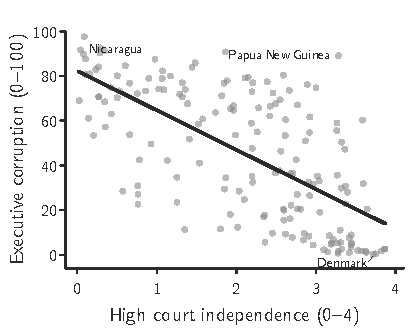
\includegraphics[width=\linewidth]{corr_court.pdf}
    \end{figure}
    \end{overprint}
    \end{column}

\end{columns}
\medskip
Interpretation: \pause Countries whose top court is rated one point more independent have, on average, $17.7$ points less executive corruption. This compares countries. It does not show that independent courts reduce corruption.
\end{frame}


\begin{frame}[t]
\frametitle{Simple Regression of Corruption on Court Independence}
\begin{columns}[T]

    \begin{column}[T]{8cm}
    \begin{footnotesize}
    \begin{itemize}
    \item But we can use more
    information in our prediction
    equation.\bigskip
    \uncover<2->{\item For example, some countries are democracies
    and others are not:}\medskip
    \begin{itemize}\begin{footnotesize}
    \uncover<3->{\item Democracies tend to have lower levels of corruption} \medskip
    \uncover<4->{\item Autocracies tend to have higher levels of corruption}
    \end{footnotesize}\end{itemize}

    \end{itemize}
    \end{footnotesize}
    \end{column}

    \begin{column}[T]{7cm}
    \begin{overprint}
    \onslide<1,2|handout:0>
    \begin{figure}[ht] \centering
        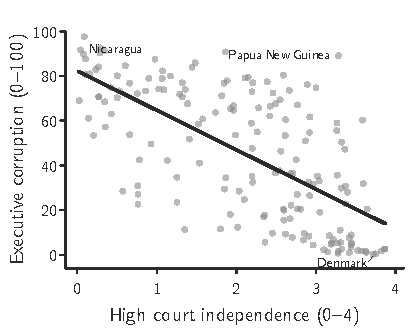
\includegraphics[width=\linewidth]{corr_court.pdf}
\end{figure}
    \onslide<3|handout:0>
    \begin{figure}[ht] \centering
        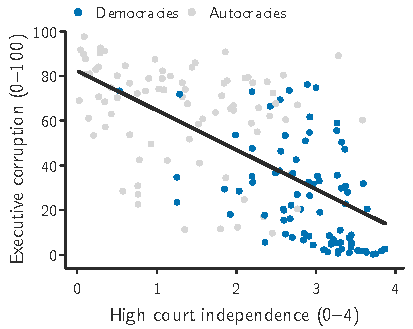
\includegraphics[width=\linewidth]{corr_court_dem.pdf}
\end{figure}
    \onslide<4|handout:1>
    \begin{figure}[ht] \centering
        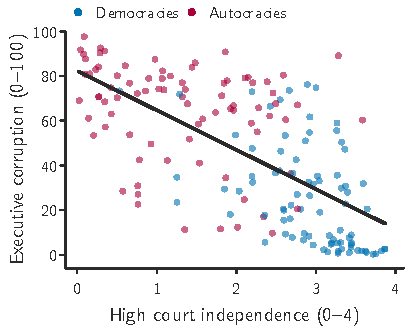
\includegraphics[width=\linewidth]{corr_court_groups.pdf}
\end{figure}
    \end{overprint}
    \end{column}

\end{columns}
\end{frame}


\frame{
\frametitle{Adding a Covariate}
\small
How do we do this? We can generalize the prediction equation:
$$
\widehat{y}_i = \widehat{\beta}_0 + \widehat{\beta}_1 x_{1i} + \widehat{\beta}_2 x_{2i}
$$
This implies that we want to predict $y$ using the information we
have about $x_1$ and $x_2$, and we are assuming a linear functional
form.\\ \pause \bigskip

Notice that now we write $X_{ji}$ where:
\begin{itemize}
  \item  $j=1,...,k$ is the index for the explanatory variables\pause
  \item $i=1,...,n$ is the index for the observation \pause
  \item we often omit $i$ to avoid clutter\\\bigskip \pause
\end{itemize}

In words:
$$
\widehat{Corruption} = \widehat{\beta}_0 + \widehat{\beta}_1\, Court + \widehat{\beta}_2\, Democracy
$$


}

\frame{
\frametitle{Interpreting a Binary Covariate}
\textbf{Worksheet Q1}

Suppose
\[
\widehat{y}=\hat\beta_0+\hat\beta_1 x_1+\hat\beta_2 x_2,\qquad
(\hat\beta_0,\hat\beta_1,\hat\beta_2)=(78.3,\,-10.6,\,-21.5),
\]
where $y$ is executive corruption (0--100), $x_1$ is high court independence (0--4), and $x_2\in\{0,1\}$ indicates democracy.\\ \bigskip

\begin{enumerate}\itemsep0.5em
  \item For a fixed level of court independence $x_1$, compute the predicted difference $\widehat{y}(x_2=1)-\widehat{y}(x_2=0)$ and interpret.
  \item For a fixed regime type, compute the predicted change when $x_1$ increases by one unit.
  \item Verify that the slope on court independence is the same in both groups and explain why.
\end{enumerate}\pause\bigskip

We are fitting two lines with the \alert{same slope} but
\alert{different intercepts}.
}

% \frame{
% \frametitle{Interpreting a Binary Covariate}

% Assume $X_{2i}$ indicates whether country $i$ used to
% be a British colony.\\\bigskip

% When $X_2=0$, the model becomes:\pause
% \begin{align*}
% \widehat{y} &= \widehat{\beta}_0 + \widehat{\beta}_1 x_{1} + \widehat{\beta}_2 \, 0 \\
%     &=  \widehat{\beta}_0 + \widehat{\beta}_1 x_{1}
% \end{align*}\pause
% When $X_2=1$, the model becomes:\pause
% \begin{align*}
% \widehat{y} &= \widehat{\beta}_0 + \widehat{\beta}_1 x_{1} + \widehat{\beta}_2 \, 1 \\
%     &=  (\widehat{\beta}_0 + \widehat{\beta}_2) + \widehat{\beta}_1 x_{1}
% \end{align*}
% What does this mean? \pause We are fitting two lines with the \alert{same slope} but
% \alert{different intercepts}.

% }


\begin{frame}[fragile]
\frametitle{Regression of Corruption on Court Independence and Democracy}
\begin{columns} [T]
\begin{column}[]{8cm}
From R, we obtain estimates $\widehat{\beta}_0,\, \widehat{\beta}_1,\, \widehat{\beta}_2$:
\begin{footnotesize}
\begin{Verbatim}[frame=single, xleftmargin=1cm, xrightmargin=1cm]
Coefficients:
            Estimate
(Intercept)  78.3236
courtind    -10.6301
democracy   -21.5101
\end{Verbatim}
\begin{itemize}
\uncover<2->{\item Autocracies:
\begin{align*}
\widehat{y} &= \widehat{\beta}_0 + \widehat{\beta}_1 x_{1}\\
\widehat{y} &= 78.3 - 10.6 \,x_{1}
\end{align*}
}
\uncover<3->{\item Democracies:
\begin{align*}
\widehat{y} &= (\widehat{\beta}_0 + \widehat{\beta}_2) + \widehat{\beta}_1 x_{1}\\
\widehat{y} &= 56.8 - 10.6\, x_{1}
\end{align*}
}
\end{itemize}
\end{footnotesize}
\end{column}
\begin{column}[]{7cm}
\begin{overprint}
\onslide<1|handout:0>
\begin{figure}[ht] \centering
        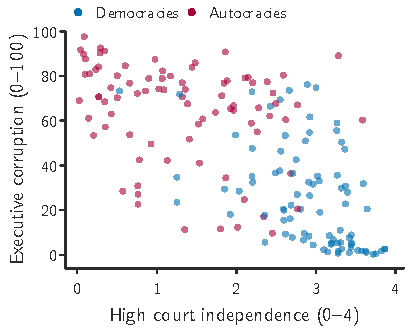
\includegraphics[width=\linewidth]{dem_points.pdf}
\end{figure}
\onslide<2|handout:0>
\begin{figure}[ht] \centering
        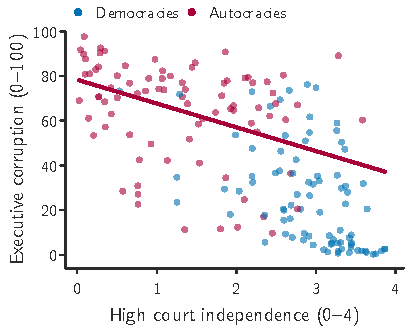
\includegraphics[width=\linewidth]{dem_line0.pdf}
\end{figure}
\onslide<3|handout:1>
\begin{figure}[ht] \centering
        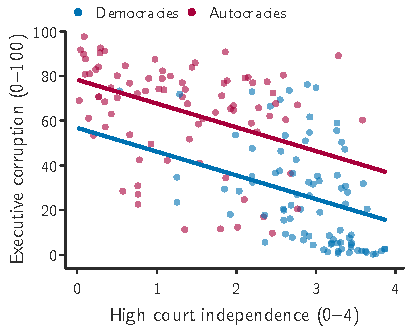
\includegraphics[width=\linewidth]{dem_lines.pdf}
\end{figure}
\end{overprint}

\end{column}
\end{columns}
\end{frame}


\frame{
\frametitle{Regression of Corruption on Court Independence and Democracy}
\begin{columns} [T]
\begin{column}[]{8cm}
Our prediction equation is:
$\widehat{y} = 78.3 - 10.6\, x_1 - 21.5 \, x_2$\\\bigskip
Where do these quantities
appear on the graph?
\begin{footnotesize}
\begin{itemize}
\uncover<2->{\item $\widehat{\beta}_0=78.3$ is the
intercept for the prediction line for autocracies.
}
\uncover<3->{\item $\widehat{\beta}_1=-10.6$ is the slope for
both lines.
}
\uncover<4->{\item $\widehat{\beta}_2=-21.5$ is the vertical
distance between the lines for democracies and autocracies.
\item Adding democracy shrinks the slope on court independence by about 40\%, from $-17.7$ to $-10.6$. Democracies have more independent courts (2.9 vs.\ 1.3 on average) and less corruption, so part of the simple slope reflects democracy.
}
\end{itemize}
\end{footnotesize}
\end{column}
\begin{column}[]{7cm}
\begin{overprint}
\onslide<1|handout:0>
\begin{figure}[ht] \centering
        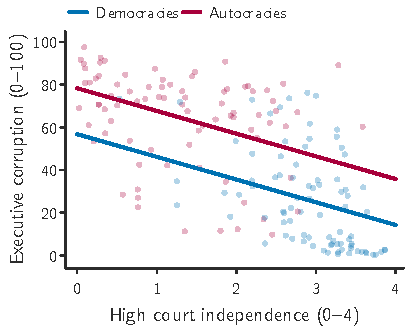
\includegraphics[width=\linewidth]{dem_zoom_lines.pdf}
\end{figure}
\onslide<2|handout:0>
\begin{figure}[ht] \centering
        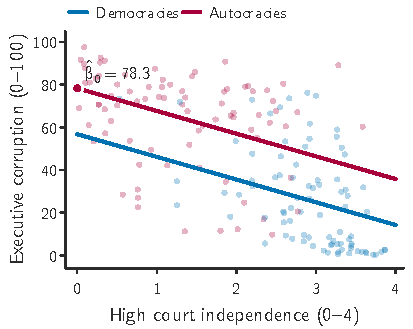
\includegraphics[width=\linewidth]{dem_zoom_b0.pdf}
\end{figure}
\onslide<3|handout:0>
\begin{figure}[ht] \centering
        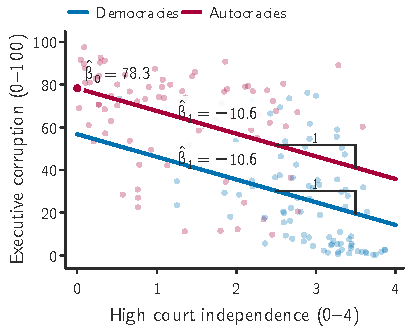
\includegraphics[width=\linewidth]{dem_zoom_b1.pdf}
\end{figure}
\onslide<4|handout:1>
\begin{figure}[ht] \centering
        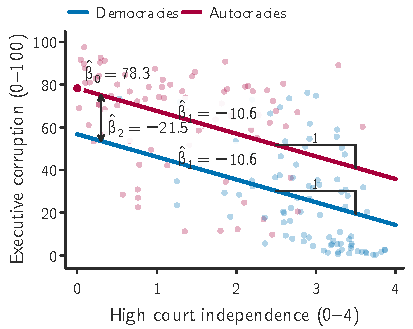
\includegraphics[width=\linewidth]{dem_zoom_b2.pdf}
\end{figure}

\end{overprint}

\end{column}
\end{columns}
}

% \frame{
% \frametitle{``Controlling'' for other variables}
% \small
% \begin{enumerate}
%   \item What difference in the democracy score do we predict between an ex-British
% colony with \alert{$Income = 3$} and an ex-British colony with \alert{$Income=2$}?\\\medskip\pause
% $\left(\widehat{\beta}_0 + \widehat{\beta}_1 (x_{1}=3)+\widehat{\beta}_2 (x_{2}=1)\right)-\left(\widehat{\beta}_0 + \widehat{\beta}_1 (x_{1}=2)+\widehat{\beta}_2 (x_{2}=1)\right)$\\
% $(-1.5+1.7\cdot 3 + 0.58\cdot 1)- (-1.5+1.7\cdot 2 + 0.58\cdot 1)= \alert{1.7}$\pause
% \item What difference in the democracy score do we predict between an non-colony with \alert{$Income = 3$} and a non-colony with \alert{$Income=2$}?\\\medskip\pause
% $\left(\widehat{\beta}_0 + \widehat{\beta}_1 (x_{1}=3)+\widehat{\beta}_2 (x_{2}=0)\right)-\left(\widehat{\beta}_0 + \widehat{\beta}_1 (x_{1}=2)+\widehat{\beta}_2 (x_{2}=0)\right)$\\
% $(-1.5+1.7\cdot 3 + 0.58\cdot 0)- (-1.5+1.7\cdot 2 + 0.58\cdot 0)= \alert{1.7}$
% \end{enumerate}\pause
% So then what do we mean by ``controlling'' for British colonial status?\\\bigskip \pause
% $\widehat{\beta}_1=1.7$ is the expected difference in the average level of democracy for countries that differ by one unit on Income, \alert{but are the same on the British colony variable}.
% }

\subsection{Multiple Regression with a Continuous Covariate}


\frame{
\frametitle{Fitting a regression plane}
\begin{columns} [c]
\begin{column}[]{8cm}
%\begin{footnotesize}
\begin{itemize}
\uncover<1->{\item We have considered an
example of multiple regression
with one \alert{continuous}
explanatory variable and one
\alert{binary} explanatory variable.\bigskip
}
\uncover<2->{\item This is easy to represent
graphically in \alert{two dimensions}
because we can use colors to
distinguish the two groups in
the data.
}
\end{itemize}
%\end{footnotesize}
\end{column}
\begin{column}[]{7cm}
\begin{overprint}
\onslide<1,2>
\begin{figure}[ht] \centering
        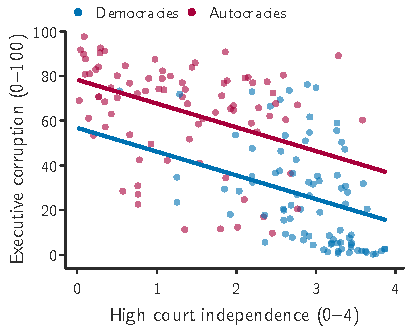
\includegraphics[width=\linewidth]{dem_lines.pdf}
\end{figure}
\end{overprint}

\end{column}
\end{columns}
}



\frame{
\frametitle{Regression of Corruption on Court Independence and Democracy}
\begin{columns} [c]
\begin{column}[]{9cm}
\begin{itemize}
\uncover<1->{\item These observations are
actually located in a
\alert{three-dimensional} space.
}
\uncover<2->{\item We can try to represent this
using a \alert{3D scatterplot}.
}
\uncover<3->{\item In this view, we are looking at
the data from the \alert{court-independence side};
the two regression lines are
drawn in the appropriate
locations.
}
\end{itemize}
\end{column}
\begin{column}[]{6cm}
\begin{overprint}
\onslide<1,2,3|handout:1>
\begin{figure}[ht] \centering
        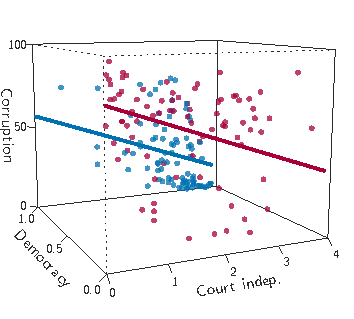
\includegraphics[width=\linewidth]{dem_3d_court.pdf}
\end{figure}
\end{overprint}

\end{column}
\end{columns}
}

\frame{
\frametitle{Regression of Corruption on Court Independence and Democracy}
\begin{columns} [c]
\begin{column}[]{9cm}
\begin{itemize}
\uncover<1->{\item We can also look at the 3D
scatterplot from the \alert{democracy side}.
}
\uncover<2->{\item While the democracy
variable is either 0 or 1, there is
nothing in the prediction
equation that requires this to be
the case.
}
\uncover<3->{\item In fact, the prediction equation
defines a \alert{regression plane} that
connects the lines when $x_2 = 0$
and $x_2 = 1$.
}
\end{itemize}
\end{column}
\begin{column}[]{6cm}
\begin{overprint}
\onslide<1,2|handout:0>
\begin{figure}[ht] \centering
        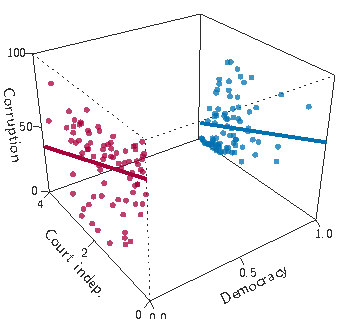
\includegraphics[width=\linewidth]{dem_3d_side.pdf}
\end{figure}
\onslide<3|handout:1>
\begin{figure}[ht] \centering
        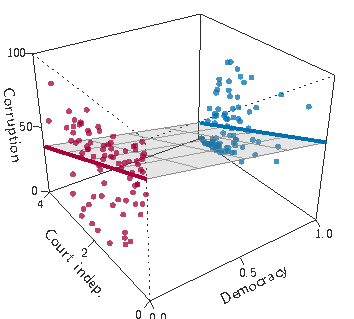
\includegraphics[width=\linewidth]{dem_3d_plane.pdf}
\end{figure}
\end{overprint}

\end{column}
\end{columns}
}


\frame{
\frametitle{Regression with two continuous variables}

\begin{itemize}
  \item Since we fit a regression plane to the data whenever we have
two explanatory variables, it is easy to move to a case with \alert{two
continuous} explanatory variables.\bigskip \pause
  \item For example, we might want to use:\\
 \begin{itemize}
    \item $X_1$ Court independence and $X_2$ $\log_{10}$ GDP per capita
    \item $Y$ Corruption
  \end{itemize}
\end{itemize}\bigskip
  $$
  \widehat{\mbox{Corruption}} = \hat\beta_0 + \hat\beta_1 \mbox{Court} +
  \hat\beta_2 \log_{10}\mbox{GDP}
  $$
}

\frame{
\frametitle{Regression of Corruption on Court Independence and GDP}

\begin{columns} [c]
\begin{column}[]{9cm}
\begin{itemize}
\uncover<1->{\item We can plot the points in a 3D
scatterplot.
}
\uncover<2->{\item R returns:
\begin{itemize}
  \item $\widehat{\beta}_{0}=166.4$
  \item $\widehat{\beta}_{1}=-13.95$ for Court independence
  \item $\widehat{\beta}_{2}=-22.0$ for $\log_{10}$ GDP per capita
\end{itemize}How does this look graphically?

}
\uncover<3->{\item These estimates define a
\alert{regression plane} through the
data.
}
\uncover<4->{\item Turned so that court independence runs left to right, the plane slopes down in that direction too.
}
\end{itemize}
\end{column}
\begin{column}[]{6cm}
\begin{overprint}
\onslide<1,2|handout:0>
\begin{figure}[ht] \centering
        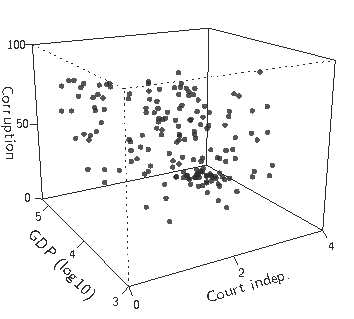
\includegraphics[width=\linewidth]{gdp_3d_points.pdf}
\end{figure}
\onslide<3|handout:0>
\begin{figure}[ht] \centering
        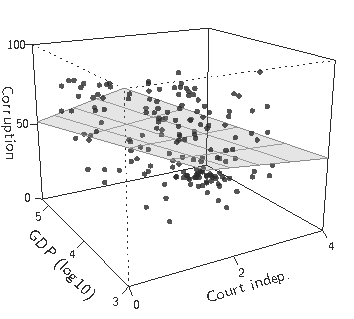
\includegraphics[width=\linewidth]{gdp_3d_plane.pdf}
\end{figure}
\onslide<4|handout:1>
\begin{figure}[ht] \centering
        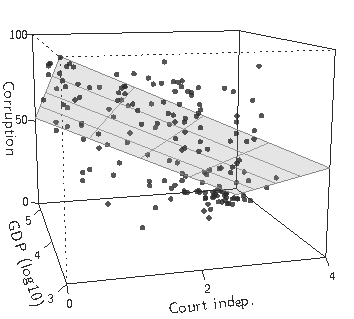
\includegraphics[width=\linewidth]{gdp_3d_rotated.pdf}
\end{figure}
\end{overprint}

\end{column}
\end{columns}
}

\frame{
\frametitle{Interpreting a Continuous Covariate}

\begin{itemize}
  \item The coefficient estimates have a similar interpretation in this
case as they did in the court independence and democracy example.\bigskip \pause
  \item For example, $\widehat{\beta}_{1}=-13.95$ represents our prediction of the difference in Corruption between two countries that differ by one point of
court independence \alert{but have the same GDP per capita}.\bigskip
\item The slope estimates have \alert{partial effect} or \alert{ceteris paribus} interpretations:
$$
\frac{\partial \widehat{y}}{\partial x_1}=\widehat{\beta}_1, \quad \widehat{y}=\widehat{\beta}_0+\widehat{\beta}_1 x_1+\widehat{\beta}_2 x_2
$$
\end{itemize}

}

\frame{
\frametitle{Interpreting a Continuous Covariate}
\begin{columns} [c]
\begin{column}[]{9cm}
\begin{itemize}
\uncover<1->{\item Again, we can think of this as
defining a regression line for
the relationship between
Corruption and Court independence at
every level of GDP per capita.
}
\uncover<2->{\item All of these lines are parallel
since they have the slope $\widehat{\beta}_{1}=-13.95$.
}
\uncover<3->{\item The lines shift down
as GDP per capita rises.
}
\end{itemize}
\end{column}
\begin{column}[]{6cm}
\begin{overprint}
\onslide<1|handout:0>
\begin{figure}[ht] \centering
        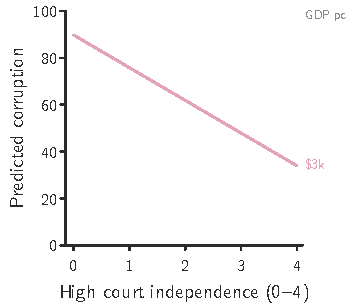
\includegraphics[width=\linewidth]{gdp_lines_1.pdf}
\end{figure}
\onslide<2|handout:0>
\begin{figure}[ht] \centering
        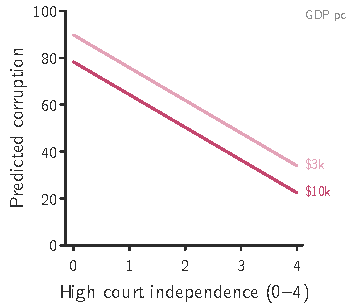
\includegraphics[width=\linewidth]{gdp_lines_2.pdf}
\end{figure}
\onslide<3|handout:0>
\begin{figure}[ht] \centering
        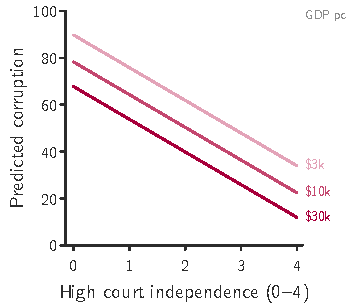
\includegraphics[width=\linewidth]{gdp_lines_3.pdf}
\end{figure}
\onslide<4|handout:1>
\begin{figure}[ht] \centering
        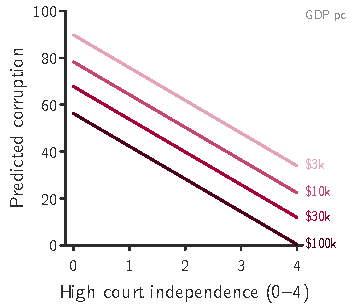
\includegraphics[width=\linewidth]{gdp_lines_4.pdf}
\end{figure}

\end{overprint}

\end{column}
\end{columns}
}

\frame{
\frametitle{More Complex Predictions}
\textbf{Worksheet Q2}\\ \medskip

With two continuous covariates, suppose
\[
\widehat{y}=\hat\beta_0+\hat\beta_1 x_1+\hat\beta_2 x_2,\qquad
(\hat\beta_0,\hat\beta_1,\hat\beta_2)=(166.4,\,-13.95,\,-22.0),
\]
where $y$ is executive corruption (0--100), $x_1$ is high court independence (0--4), and $x_2$ is $\log_{10}$ GDP per capita.
\begin{enumerate}\itemsep0.5em
\item Show that for any two units $A$ and $B$,
\[
\widehat{y}_A-\widehat{y}_B=\hat\beta_1(x_{1A}-x_{1B})+\hat\beta_2(x_{2A}-x_{2B}).
\]
\item Using $(x_1,x_2)=(2.96,\,4.48)$ for Chile and $(0.21,\,4.38)$ for China, compute the predicted levels and their difference.  
\item Explain the ``partial effect'' meaning of $\hat\beta_1$ and $\hat\beta_2$.
\end{enumerate}
}



% \frame{
% \frametitle{More Complex Predictions}

% \begin{itemize}
%   \item We can also use the coefficient estimates for more complex predictions that involve changing multiple variables simultaneously.\medskip \pause
%   \item Consider our results for the regression of democracy on $X_1$ income and $X_2$ ethnic heterogeneity:
%   \begin{itemize}
%   \item $\widehat{\beta}_{0}=-.71$
%   \item $\widehat{\beta}_{1}=1.6$
%   \item $\widehat{\beta}_{2}=-.6$
%   \end{itemize}\medskip
% \item What is the predicted difference in democracy between
%  \begin{itemize}
%    \item \alert{Chile} with $X_1=3.5$ and $X_2=.06$
%    \item \alert{China} with $X_1=2.5$ and $X_2=.5$?
%  \end{itemize}\pause
% \item Predicted democracy is
% \begin{itemize}
%   \item $-.71 + 1.6 \cdot 3.5 -.6 \cdot .06=4.9$ for \alert{Chile}\\\pause
%   \item $-.71 + 1.6 \cdot 2.5 -.6 \cdot .5=3$ for \alert{China}.\\\pause
% \end{itemize}
% Predicted difference is thus: $1.9$ or $(3.5-2.5)\widehat{\beta}_{1}+(.06-.5)\widehat{\beta}_{2}$
% \end{itemize}

% % Talk about ATE (averaging over X) here?

% }


\section{Mechanics of Multiple Regression}


\subsection{Derivation and Properties of OLS Estimator}

\frame{
\frametitle{Deriving the Linear Least Squares Estimator}
\begin{itemize}
\item In simple regression, we chose $(\widehat{\beta}_0, \widehat{\beta}_1)$ to minimize the
sum of the squared residuals

\item We use the same principle for picking $(\widehat{\beta}_0,
  \widehat{\beta}_1, \widehat{\beta}_2)$ for regression with two
  regressors ($x_i$ and $z_i$):
\begin{eqnarray*}
    (\hat{\beta}_0, \hat{\beta}_1, \hat{\beta}_2)  & = &
     \underset{\tilde{\beta}_0, \tilde{\beta}_1, \tilde{\beta}_2}{\textrm{argmin}}
    \sum_{i=1}^n (y_i - \tilde{\beta}_0 - x_i \tilde{\beta}_1 - z_i \tilde{\beta}_2)^2
\end{eqnarray*}
\pause

\item (The same works more generally for $k$
  regressors, but this is done more easily with matrices as we see later)

\end{itemize}

}


\frame{
\frametitle{Deriving the Linear Least Squares Estimator}
We want to minimize the following quantity with respect to
$(\tilde\beta_0, \tilde\beta_1, \tilde\beta_2)$:
$$
S(\tilde{\beta}_0, \tilde{\beta}_1, \tilde{\beta}_2) = \sum_{i=1}^n (y_i -
\tilde{\beta}_0 - \tilde{\beta}_1 x_i - \tilde{\beta}_2 z_i)^2
$$

How do we proceed?\pause
\begin{enumerate}
  \item  Take the partial derivatives of $S$ with respect to
    $\tilde{\beta}_0, \tilde{\beta}_1$ and $\tilde{\beta}_2$.\medskip\pause
  \item Set each of the partial derivatives to 0 to obtain the \alert{first order conditions}.\medskip\pause
  \item Substitute $\hat{\beta}_0, \hat{\beta}_1,\hat{\beta}_2$ for
    $\tilde{\beta}_0, \tilde{\beta}_1,\tilde{\beta}_2$ and solve for
    $\hat{\beta}_0, \hat{\beta}_1,\hat{\beta}_2$ to obtain the OLS estimator.
\end{enumerate}

}

\frame{
\frametitle{First Order Conditions}
\small
 Setting the partial derivatives equal to zero leads to a system of
  $3$ linear equations in $3$ unknowns: $\hat{\beta}_0,
  \hat{\beta}_1$ and $\hat{\beta}_2$
\begin{eqnarray*}
-\frac{1}{2}\frac{\partial S}{\partial \tilde{\beta}_0 }\Big|_{\tilde\beta=\hat\beta} & = & \sum_{i=1}^n (y_i -
\hat{\beta}_0 - \hat{\beta}_1 x_i - \hat{\beta}_2 z_i ) \ = \ 0\\
-\frac{1}{2}\frac{\partial S}{\partial \tilde{\beta}_1 }\Big|_{\tilde\beta=\hat\beta} & = & \sum_{i=1}^n
x_i(y_i - \hat{\beta}_0 - \hat{\beta}_1 x_i - \hat{\beta}_2 z_i) \ = \ 0\\
-\frac{1}{2}\frac{\partial S}{\partial \tilde{\beta}_2 }\Big|_{\tilde\beta=\hat\beta} & = & \sum_{i=1}^n
z_i(y_i - \hat{\beta}_0 - \hat{\beta}_1 x_i - \hat{\beta}_2 z_i) \ = \ 0\\
\end{eqnarray*}
When will this linear system have a unique solution? \pause
\begin{itemize}
  \item More observations than predictors (i.e. $n>2$)
  \item $x$ and $z$ are \alert{linearly independent}, i.e.,
    \begin{itemize}
      \item neither $x$ nor $z$ is a constant
      \item $x$ is not a linear function of $z$ (or vice versa)
    \end{itemize}
  \item Wooldridge calls this assumption \alert{no perfect collinearity}
\end{itemize}
}

\frame{
\frametitle{The OLS Estimator}
\small
The OLS estimators of $(\beta_0, \beta_1, \beta_2)$ can be written as
\begin{eqnarray*}
\hat{\beta}_0 & = & \bar{y} - \hat{\beta}_1 \bar{x} - \hat{\beta}_2 \bar{z} \\
\hat{\beta}_1
% & = & \frac{\sum_{i=1}^n x_i^{*} y_i^{*}\sum_{i=1}^n z_i^{*2} -
% \sum_{i=1}^n z_i^{*} y_i^{*}\sum_{i=1}^n x_i^{*}z_i^{*} }{\sum_{i=1}^n
% x_i^{*2} \sum_{i=1}^n z_i^{*2} - (\sum_{i=1}^n x_i^{*} z_i^{*})^2} \\
             & = & \frac{Cov(x,y)Var(z) - Cov(z,y)Cov(x,z)}{Var(x)Var(z) - Cov(x,z)^2} \\
\hat{\beta}_2
% & = & \frac{\sum_{i=1}^n z_i^{*} y_i^{*}\sum_{i=1}^n
% x_i^{*2} - \sum_{i=1}^n x_i^{*} y_i^{*}\sum_{i=1}^n z_i^{*}x_i^{*}
% }{\sum_{i=1}^n x_i^{*2} \sum_{i=1}^n z_i^{*2} - (\sum_{i=1}^n x_i^{*}
% z_i^{*})^2} \\
   & = & \frac{Cov(z,y)Var(x) - Cov(x,y)Cov(z,x)}{Var(x)Var(z) - Cov(x,z)^2}
\end{eqnarray*}
where $Var$, $Cov$, $Cor$ are sample moments.

\pause
For $(\hat\beta_0,\hat\beta_1,\hat\beta_2)$ to be well-defined we need:
$$
Var(x) Var(z) \ne Cov(x,z)^2
$$
Condition fails if:\pause
\begin{enumerate}
  \item If $x$ or $z$ is a constant ($\Rightarrow$ $Var(x)Var(z) = Cov(x,z) = 0$)
  \item One explanatory variable is an exact linear function of another
    ($\Rightarrow \ |Cor(x,z)|=1 \ \Rightarrow \ Var(x)Var(z) = Cov(x,z)^2$)
\end{enumerate}

}

\frame{
\frametitle{Important Properties of OLS Estimator}

\textbf{Worksheet Q3}
Analogous to the single variable case, show that the fitted values and residuals have three important properties:\bigskip\pause
\begin{enumerate}\itemsep1em
  \item $\sum_{i=1}^n \hat{u}_i=0$. 
%  Proof: $\bar{\hat{u}} = \bar{y} - \hat\beta_0 - \hat\beta_1 \bar{x} - \hat\beta_2\bar{z} = \bar{y} - (\bar{y}-\hat\beta_1 \bar{x} - \hat\beta_2\bar{z}) - \hat\beta_1 \bar{x} - \hat\beta_2\bar{z} =0$
$\Rightarrow \bar{y}=\bar{\hat{y}}$.
%  Proof: $y_i = \hat{y}_i + \hat{u}_i$ so $\bar{y}=n^{-1}\sum_{i=1}^n y_i=n^{-1}\sum_{i=1}^n (\hat{y}_i + \hat{u}_i)=\bar{\hat{y}}-\bar{\hat{u}}=\bar{\hat{y}}$
\item The point ($\bar{y}, \bar{x},\bar{z}$) is always on the regression plane.
\item $Cov(x,\hat{u})=Cov(z,\hat{u})=0$. $\Rightarrow Cov(\hat{y},\hat{u})=0$.
%  $\sum_{i=1}^n \hat{u}_i x_{i,1}=\sum_{i=1}^n (y_i - \beta_1 x_{i,1})x_{i,1}=\sum_{i=1}^n  y_i x_{i,1} - \beta_1 \sum_{i=1}^n x^2_{i,1}= \sum_{i=1}^n  y_i x_{i,1} -\sum_{i=1}^n  y_i x_{i,1}$ (sub in for $\beta_1$)
\bigskip

\end{enumerate}
}

\subsection{Analysis of Variance}

\frame{
\frametitle{Fitted Values and Residuals}
\begin{columns} [c]
\begin{column}[]{9cm}
\begin{itemize}
\uncover<1->{\item We can define \alert{fitted values} and
\alert{residuals} as we did in simple
linear regression:
}
\uncover<2->{\item Fitted Values:\\
$\widehat{y}_i = \widehat{\beta}_0 + \widehat{\beta}_1 x_{1i} + \widehat{\beta}_2 x_{2i}$ \\
for $i=1,...,n$
}
\uncover<3->{\item Residuals:\\
$\widehat{u}_i = y_i - \widehat{y}_i$\\
for $i=1,...,n$
}
\uncover<4->{\item The residuals are the vertical
distance between the
observation and the regression
plane.
\item Corruption cannot fall below 0. Rich democracies such as Denmark (0.3) and Sweden (0.4) sit on this floor, about 7 to 8 points below the plane.
}
\end{itemize}
\end{column}
\begin{column}[]{6cm}
\begin{overprint}
\onslide<1,2,3|handout:0>
\begin{figure}[ht] \centering
        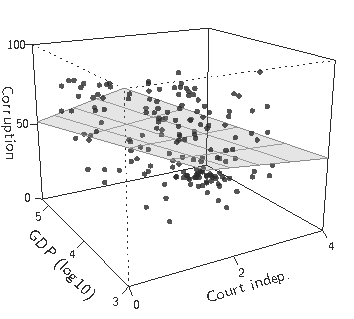
\includegraphics[width=\linewidth]{gdp_3d_plane.pdf}
\end{figure}
\onslide<4|handout:1>
\begin{figure}[ht] \centering
        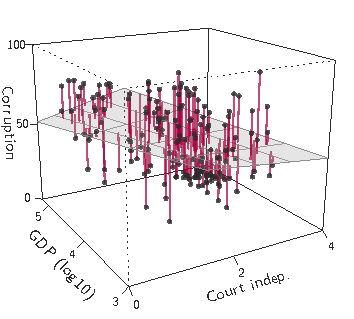
\includegraphics[width=\linewidth]{gdp_3d_resid.pdf}
\end{figure}
\end{overprint}

\end{column}
\end{columns}
}

% \frame{
% \frametitle{Extending beyond two independent variables}

% \begin{itemize}
% \item We can extend this concept of conditioning on additional variables to include $k$ independent variables.\medskip
% \item Conceptually similar: the data will form a $k+1$ dimensional data cloud, and the least squares estimator will be a $k$ dimensional hyperplane through this cloud that minimizes the sum of the squared residuals.\medskip
% \item Unfortunately, we can't plot these objects, but we can imagine what they might look like by thinking about the transition from simple regression to two independent variable regression.
% \end{itemize}

% }

\frame{
\frametitle{Analysis of Variance for Multiple Regression}
\small
%Notice that regression implies a decomposition of the variance into three parts.
\begin{columns}[]
\begin{column}[]{8cm}
\centering
\begin{itemize}
\uncover<1->{
\item $\sum_{i}^n (y_i - \bar{y})^2 = \mbox{SST}$\\ \alert{(Total Sum of Squares)} \medskip}
\uncover<2->{
\item $\sum_{i}^n (\hat{y}_i - \bar{y})^2 = \mbox{SSE} $ \\ \alert{(Explained Sum of Squares)} \medskip}
\uncover<3->{
\item $\sum_{i}^n (\hat{y}_i - y_i)^2 = \sum_{i}^n \hat{u}_i^2 = \mbox{SSR} $ \\ \alert{(Residual Sum of Squares)} \medskip
}
\end{itemize}
\end{column}
\begin{column}[]{7cm}
\begin{overprint}
\onslide<1|handout:0>
\begin{figure}[ht] \centering
        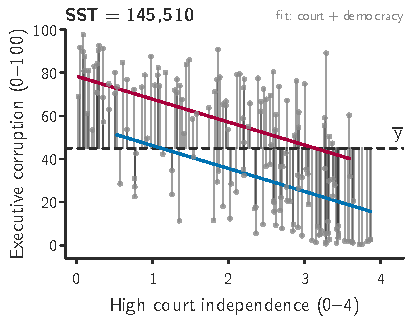
\includegraphics[width=\linewidth]{anova_sst.pdf}
\end{figure}
\onslide<2|handout:0>
\begin{figure}[ht] \centering
        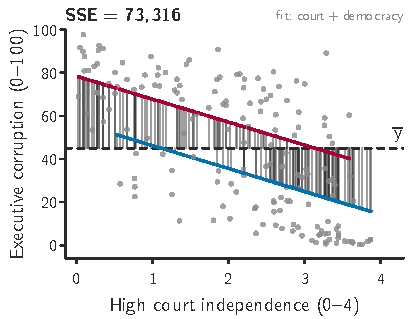
\includegraphics[width=\linewidth]{anova_sse.pdf}
\end{figure}
\onslide<3|handout:1>
\begin{figure}[ht] \centering
        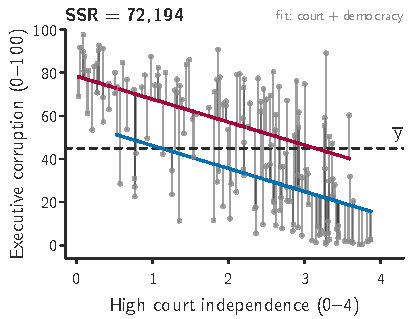
\includegraphics[width=\linewidth]{anova_ssr.pdf}
\end{figure}
\end{overprint}
\end{column}
\end{columns}
}
%\frame{
%\frametitle{Coefficient of Determination $r^2$}
%
%Given $SST = SSE + SSR$ we can divide each side by the $SST$:
%
%$$
%\frac{SST}{SST} = \frac{SSE}{SST} + \frac{SSR}{SST}
%$$
%%$$
%%1 = \frac{SSE}{SST} + \frac{SSR}{SST}
%%$$
%$$
%r^2 = 1 - \frac{SSR}{SST} = \frac{SSE}{SST}
%$$
%$$
%r^2 =\frac{\sum_i^n ((y_i - \bar{y})(\hat{y}_i - \bar{y}))^2   }{(\sum_i^n (y_i - \bar{y})^2   )(\sum_i^n (\hat{y}_i - \bar{y})^2  )}
%$$
%$$
%0 \leq r^2 \leq 1  \mbox { and also } r^2=(r)^2
%$$\\\medskip
%
%
%
%Notice that compared to the bivariate case we saw last week, nothing has changed except our definition of $\hat{y}_i$.
%
%}
%
%\frame{
%\frametitle{Questions about $r^2$}
%
%Which of the following statements about $r^2$ is incorrect?
%\begin{enumerate}
%  \item If $r^2=1$, then every observation in the data is predicted
%perfectly.\medskip
%  \item Including an additional variable in the model will never
%decrease $r^2$.\medskip
%  \item A high $r^2$ indicates that all of the model assumptions are
%satisfied.\medskip
%  \item $r^2=0$ iff the estimated coefficients on
%all of the explanatory variables are exactly zero.
%\end{enumerate}
%}

\frame{
\frametitle{Adjusted $R^2$}
\begin{itemize}
\item $R^2 = SSE/SST$ never decreases when a regressor is added (same observations)
\item Problematic as a criterion for \alert{model selection}
\item We may prefer a {\it parsimonious} model over a slightly worse
  fitting but much more complicated model; alternative: \alert{Adjusted $R^2$}
\item Penalizes model complexity: it multiplies $1-R^2$ by $(n-1)/(n-k-1)$, which grows with $k$

$$
\mbox{Adjusted} \, R^2 = 1 - (1- R^2)\frac{n-1}{n-k-1}
$$
Later we can show that $\mbox{Adjusted} \, R^2$ increases iff the absolute $t$–statistic on the added regressor exceeds $1$.
\medskip
\item Drawbacks:
  \begin{itemize}
  \item No longer guaranteed to be in $[0,1]$
  \item No longer directly interpretable as proportion of explained variance in $y_i$
  \end{itemize}
\end{itemize}
}

\begin{frame}[fragile]
\frametitle{Adjusted $R^2$}
\spacingset{0.8}
\begin{Verbatim}[fontsize=\footnotesize, frame=single, label=R Code, commandchars=\\\{\}]
> summary(lm(execorr100 ~ courtind + democracy, data = d))

Call:
lm(formula = execorr100 ~ courtind + democracy, data = d)

Residuals:
    Min      1Q  Median      3Q     Max
-52.662 -16.714   1.861  13.911  50.129

Coefficients:
            Estimate Std. Error t value Pr(>|t|)
(Intercept)   78.324      3.593  21.799  < 2e-16 ***
courtind     -10.630      2.113  -5.031 1.27e-06 ***
democracy    -21.510      4.672  -4.604 8.22e-06 ***
---
Signif. codes:  0 *** 0.001 ** 0.01 * 0.05 . 0.1   1

Residual standard error: 20.92 on 165 degrees of freedom
Multiple R-squared: 0.5039,	\textcolor{red}{Adjusted R-squared: 0.4978}
F-statistic: 83.78 on 2 and 165 DF,  p-value: < 2.2e-16
\end{Verbatim}
\end{frame}


\frame{
\frametitle{ANOVA Decomposition, $R^2$, and Adjusted $R^2$}
\textbf{Worksheet Q4}\\ \bigskip

Let $\hat y_i$ be fitted values from OLS with intercept and two regressors, and $\hat u_i=y_i-\hat y_i$.\\ \medskip
\begin{enumerate}\itemsep0.5em
  \item Show: SST = SSE + SSR
  \item Explain why $R^2$ is weakly increasing when a regressor is added
\end{enumerate} \bigskip
  Later we can show that the adjusted $R^2$
\[
\overline{R}^2=1-(1-R^2)\frac{n-1}{n-k-1}
\]
increases iff the absolute $t$–statistic on the added regressor exceeds $1$.

}


\subsection{``Partialling Out'' Interpretation}

\begin{frame}[t]
\frametitle{``Partialling Out'' Interpretation of the OLS Estimator}
\small
Assume $Y = \beta_0 + \beta_1 X + \beta_2 Z + u$. Another way to write the OLS estimator is:
$$
\hat{\beta}_1 = \frac{\sum_i^n \hat{r}_{xz,i}\,y_i}{\sum_i^n\hat{r}^2_{xz,i}}
$$
where $\hat{r}_{xz,i}$ are the residuals from the regression of $X$ on $Z$:
$$
x_i = \hat{\lambda} + \hat{\delta} z_i + \hat{r}_{xz,i}
$$
\pause
\vspace{-1em}\begin{itemize}
\item In other words, both of these regressions yield identical estimates $\hat{\beta}_1$ (but different fitted values $\tilde{y}$ and $\hat{y}$):
$$
\tilde{y} = \hat{\gamma}_0 + \hat{\beta}_1 \hat{r}_{xz} \quad \mbox{and} \quad \hat{y} = \hat{\beta}_0 + \hat{\beta}_1 x + \hat{\beta}_2 z
$$\pause\vspace{-1em}
\item $\hat\delta$ is the slope of that regression; it is zero exactly when $X$ and $Z$ are uncorrelated in the sample. \pause What is our estimator $\hat{\beta}_1$ if $\hat\delta=0$ in our sample? \pause

$$\hat r_{xz,i} = x_i - \hat{\lambda}= x_i - \bar{x} \quad \text{so} \quad \hat{\beta}_1 = \frac{\sum_i^n \hat{r}_{xz,i}\,y_i}{\sum_i^n\hat{r}^2_{xz,i}}= \pause \frac{\sum_i^n ( x_i - \bar{x})\,y_i}{\sum_i^n ( x_i - \bar{x})^2 }$$
That is, same as the simple regression of $Y$ on $X$ alone. 
\end{itemize}

\end{frame}


\begin{frame}[t]
\frametitle{``Partialling Out'' Interpretation of the OLS Estimator}
Both of these regressions yield identical estimates $\hat{\beta}_1$ (but different fitted values $\tilde{y}$ and $\hat{y}$):
$$
\tilde{y} = \hat{\gamma}_0 + \hat{\beta}_1 \hat{r}_{xz} \quad \mbox{and} \quad \hat{y} = \hat{\beta}_0 + \hat{\beta}_1 x + \hat{\beta}_2 z
$$
\begin{itemize}
\item Residuals $\hat{r}_{xz}$ are the part of $X$ that is uncorrelated with $Z$. Put differently, $\hat{r}_{xz}$ is $X$, after its linear association with $Z$ has been \alert{partialled out} or netted out.
\item We can use same equation with $k$ explanatory variables; $\hat{r}_{xz}$ will then come from a regression of $X$ on all the other explanatory variables.
\item We will prove this later using matrix algebra.
\end{itemize}
\end{frame}



\frame{
\frametitle{Regression: Corruption on Court Independence}
{\centering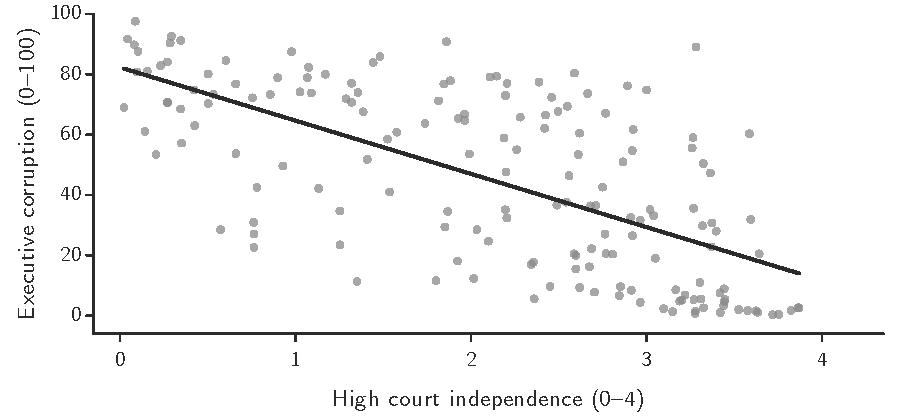
\includegraphics[height=0.70\textheight]{fwl_corr_court.pdf}\par}
$\widehat{\mbox{Corr}} = 82.3 - 17.7 \mbox{ Court}$. \pause But richer countries tend to have more independent courts, and richer countries are much less corrupt...
}

\frame{
\frametitle{Regression: Court Independence on GDP}
{\centering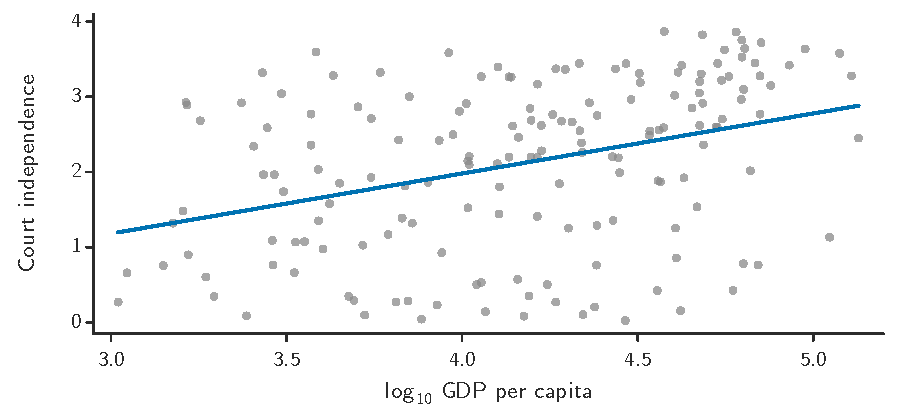
\includegraphics[height=0.70\textheight]{fwl_court_gdp.pdf}\par}
\begin{scriptsize}
...like this...
\end{scriptsize}
}

\frame{
\frametitle{Regression: Corruption on GDP}
{\centering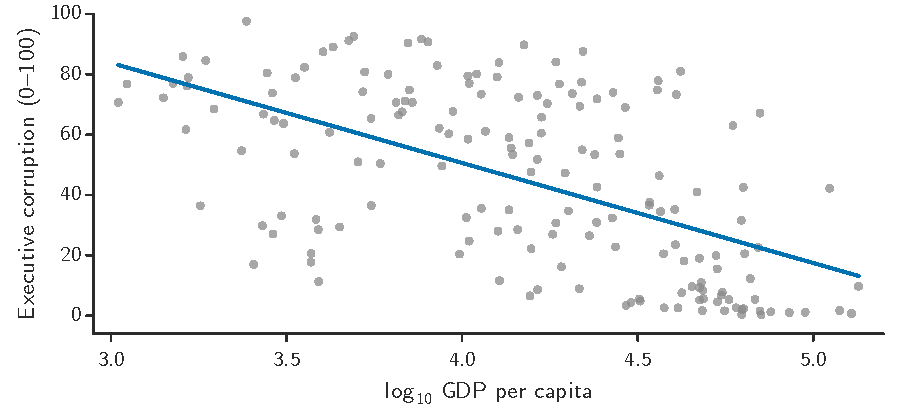
\includegraphics[height=0.70\textheight]{fwl_corr_gdp.pdf}\par}
and like this.
}


\frame{
\frametitle{Regression: Corruption on Court Independence}
{\centering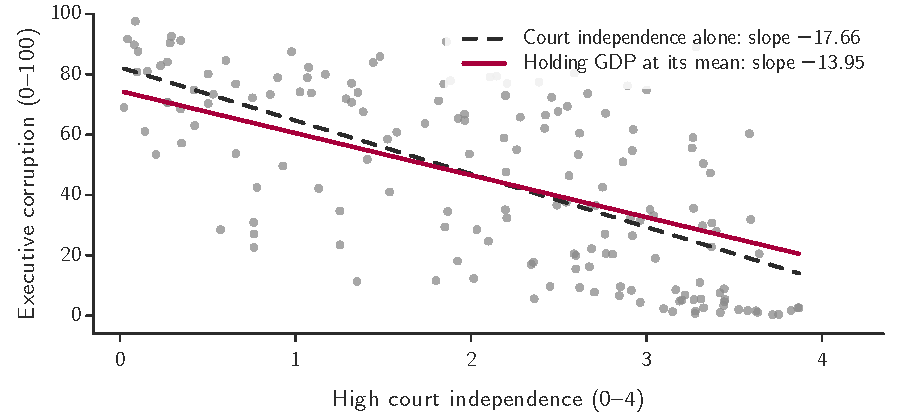
\includegraphics[height=0.70\textheight]{fwl_corr_court_partial.pdf}\par}
$\widehat{\mbox{Corr}} = 166.4 - 13.95 \mbox{ Court} - 22.0 \log_{10}\mbox{GDP}$. Holding GDP fixed, the slope shrinks from $-17.7$ to $-13.95$. Court independence tracks income only loosely ($r=0.37$), so income explains only a fifth of the slope.
}

\frame{
\frametitle{Regression: Court Independence on GDP}
{\centering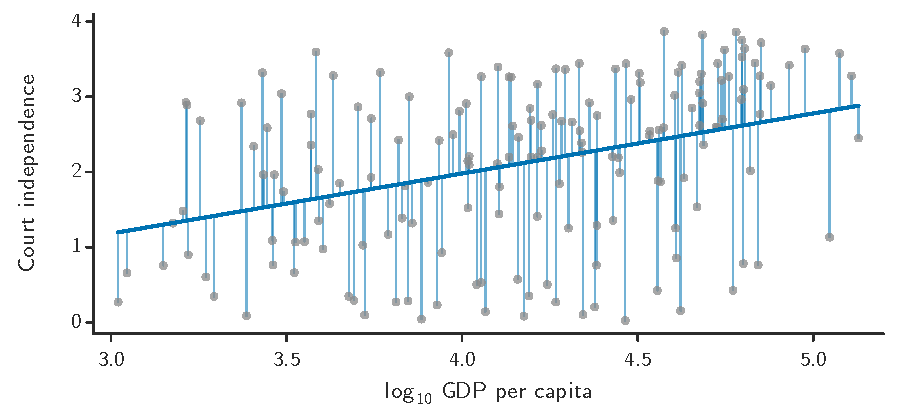
\includegraphics[height=0.70\textheight]{fwl_court_gdp_resid.pdf}\par}
$\widehat{\mbox{Court}} = -1.21 + 0.80 \log_{10}\mbox{GDP}$. The residuals from the regression of court independence on GDP measure the variation in court independence that is uncorrelated with GDP.
}

\frame{
\frametitle{Regression: Corruption on Court Independence}
{\centering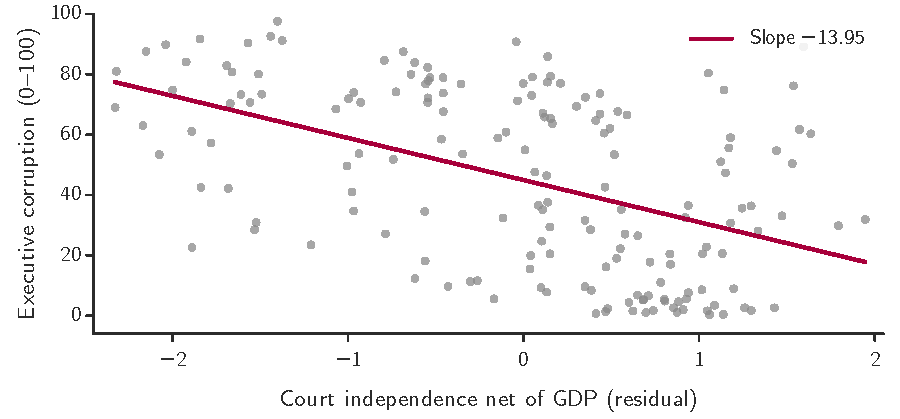
\includegraphics[height=0.70\textheight]{fwl_corr_resid.pdf}\par}
$\widehat{\mbox{Corr}} = 44.94 - 13.95 \mbox{ Res: Court on GDP}$. Regressing corruption on these residuals gives the same slope as the plane.
}

\begin{frame}[fragile]
\frametitle{Regression: Corruption on Court Independence}
\spacingset{0.8}
\begin{Verbatim}[fontsize=\footnotesize, frame=single, label=R Code, commandchars=\\\{\}]
> summary(lm(execorr100 ~ courtind, data = d))

Call:
lm(formula = execorr100 ~ courtind, data = d)

Residuals:
    Min      1Q  Median      3Q     Max
-47.164 -17.940   0.949  15.506  64.745

Coefficients:
            Estimate Std. Error t value Pr(>|t|)
(Intercept)   82.327      3.692   22.30   <2e-16 ***
courtind     -17.664      1.546  -11.42   <2e-16 ***
---
Signif. codes:  0 *** 0.001 ** 0.01 * 0.05 . 0.1   1

Residual standard error: 22.15 on 166 degrees of freedom
Multiple R-squared: 0.4401,	Adjusted R-squared: 0.4367
F-statistic: 130.5 on 1 and 166 DF,  p-value: < 2.2e-16
\end{Verbatim}

\end{frame}

\begin{frame}[fragile]
\frametitle{Regression: Court Independence on GDP}
\footnotesize
\spacingset{0.6}
\begin{Verbatim}[fontsize=\footnotesize, frame=single, label=R Code, commandchars=\\\{\}]
> d$lgdp <- log10(d$gdppc)  # log10 GDP per capita
> fit <- lm(courtind ~ lgdp, data = d)
> summary(fit)

Call:
lm(formula = courtind ~ lgdp, data = d)

Residuals:
    Min      1Q  Median      3Q     Max
-2.3267 -0.6259  0.1371  0.8021  1.9460

Coefficients:
            Estimate Std. Error t value Pr(>|t|)
(Intercept)  -1.2123     0.6604  -1.836   0.0682 .
lgdp          0.7981     0.1572   5.078 1.01e-06 ***
---
Signif. codes:  0 *** 0.001 ** 0.01 * 0.05 . 0.1   1

Residual standard error: 1.035 on 166 degrees of freedom
Multiple R-squared: 0.1345,	Adjusted R-squared: 0.1292
F-statistic: 25.79 on 1 and 166 DF,  p-value: 1.015e-06

> d$res_court_gdp <- residuals(fit)  # store residuals as a new variable
\end{Verbatim}

\end{frame}

\begin{frame}[fragile]
\frametitle{Regression: Corruption on Netted-Out Court Independence}
\spacingset{0.8}
\begin{Verbatim}[fontsize=\footnotesize, frame=single, label=R Code, commandchars=\\\{\}]
> summary(lm(execorr100 ~ courtind + lgdp, data = d))

~~~~~
Coefficients:
            Estimate Std. Error t value Pr(>|t|)
(Intercept)  166.352     12.626  13.175  < 2e-16 ***
\textcolor{red}{courtind     -13.952}      1.469  -9.497  < 2e-16 ***
lgdp         -22.028      3.198  -6.889 1.13e-10 ***
---
Signif. codes:  0 *** 0.001 ** 0.01 * 0.05 . 0.1   1
~~~~~

> summary(lm(execorr100 ~ res_court_gdp, data = d))

~~~~~
Coefficients:
              Estimate Std. Error t value Pr(>|t|)
(Intercept)     44.942      1.994  22.534  < 2e-16 ***
\textcolor{red}{res_court_gdp  -13.952}      1.939  -7.194 2.06e-11 ***
---
Signif. codes:  0 *** 0.001 ** 0.01 * 0.05 . 0.1   1
~~~~~
\end{Verbatim}
\end{frame}


%\frame{
%\frametitle{Regression: Democracy on Income and British Colony}
%
%
%\begin{figure}[ht] \centering
%        \scalebox{.65}{\includegraphics{adjrsq.pdf}}
%\end{figure}
%}
%
%\frame{
%\frametitle{Regression: Income on British Colony}
%
%
%\begin{figure}[ht] \centering
%        \scalebox{.65}{\includegraphics{addvar.pdf}}
%\end{figure}
%}
%
%\frame{
%\frametitle{Regression: Democracy on Partialled out Income}
%
%
%\begin{figure}[ht] \centering
%        \scalebox{.65}{\includegraphics{addvar2.pdf}}
%\end{figure}
%}
%
%\frame{
%\frametitle{Next Steps}
%
%\begin{itemize}
%  \item Properties of multivariate OLS estimators
%  \item Linear model assumptions
%  \item Standard errors, testing, p-values, and confidence intervals
%  \item Polynomials to Incorporate Further Non-Linearities
%  \item Interactions
%  \item F-tests
%  \item Dummy Variables
%\end{itemize}
%

%}
%
%%\begin{frame}
%%  \frametitle{Required readings}
%%Due Wednesday next week:
%%\begin{itemize}
%%\item Wooldrige: Chapter 4\\\bigskip
%%%\item Acock: Ch 5 + 6 (if you lack Stata background)
%%\end{itemize}
%%\end{frame}

\end{document}
